\chapterimage{images/chameleon.jpeg} % Chapter heading image

\chapter{Chameleon Cloud}
\label{C:chameleon}
\index{Chameleon}
/FILENAME/

\section{Overview}

\FILENAME

This chapter is copied from the Chameleon Web page. However we have
included where appropriate some updates. 

Chameleon is an experimental testbed for Computer Science funded by the
NSF FutureCloud program. Chameleon is built over two sites, University
of Chicago and TACC, offering a total of over 550 nodes and 5 PB of
space in twelve
\href{https://www.chameleoncloud.org/about/hardware-description/}{Standard
Cloud Unit (SCU) racks}. To effectively support Computer Science
experiments Chameleon offers bare metal reconfigurability on most of the
hardware. To provide easy access to educational users, three SCUs at
TACC (a quarter of the testbed) are configured with OpenStack KVM. You
can read more about
Chameleon~\href{https://www.chameleoncloud.org/about/chameleon/}{here}.

Chameleon is broadly available to members of the US Computer Science
research community and its international collaborators working in the
open community on cloud research. The expectation is that any research
performed on Chameleon will result in publication in a broadly
available journal or conference.

In order to promote fairness to all users, we have~the following set of
Best Practices for using Chameleon~bare metal partitions:

\begin{description}
\item
  \item[Think Small for Development and class use:] If you are just developing or
  prototyping a system, and not yet running experiments at scale, use
  only as many nodes as you actually need (e.g., many projects can be
  developed and tested on 3-4 nodes), and try to take short
  reservations. Start with hours first and do not let your VMs
  unnecessarily run for long unused periods. 
\item
  \item[Automate deployments:] You can always snapshot your work/images
  between sessions using the
  \href{https://www.chameleoncloud.org/docs/user-guides/ironic/\#snapshotting_an_instance}{snapshotting
  instructions} to simplify the redeployment of your environment during
  the next work session. You can also use scripting and environment
  customization to make it easier to redeploy images. An additional
  benefit of automation is that it makes it easier for you to reproduce
  your work and eventually~share it~with colleagues within your lab and
  other collaborators.
\item [Think Big for Experimentation:] Once you are ready to experiment you
  will want to test your experimental setup on increasingly larger
  scales. This is possible by taking an advance reservation for many
  resources for a relatively short time. The more resources you need,
  the more likely it is that you will need to run experiments at a less
  attractive time (e.g., during the weekend) --- here's where automation
  will also help. In justified cases, we will support reserving even the
  whole bare metal testbed.
\end{description}



\FILENAME

\section{Resources}

In any case please visit the Chameleon Web page as there is also more
information about other topics that we may not care about. Furthermore
we do not use Advanced Appliences, but use ansible instead as it is
independent from OpenStack and can be used with other frameworks.

If you prefer you can also go to the Chameleon Web site using the
following links. However we have improved some of the documentation
found in this document. We would like to get your feedback in case you
find errors or like to contribute tho this documentation.

\begin{WARNING}
  Chameleon cloud promotes insecure use of ssh while suggesting
  passphrase less keys. This is {\bf very dangerous} due to the fact
  that somone could gain access to your computer and if a password
  less key is stolen easy access to other systems can be
  achieved. INstead you must use whenever possible passphrases and use
  ssh agend and ssh add!

  Hence do not use their advise that is mantioned multiple times in
  their documentation. Follow ours!
\end{WARNING}

The links to Chameleons Documentation 

\begin{itemize}
\item
  \href{https://www.chameleoncloud.org/}{Home}
\item
  \href{openstack-kvm-user-guide.html\#}{Documentation }

  \begin{itemize}
    \item
    \href{https://www.chameleoncloud.org/docs/getting-started/}{Getting
    Started}
  \item
    \href{https://www.chameleoncloud.org/docs/bare-metal-user-guide/}{Bare
    Metal}
  \item
    \href{https://www.chameleoncloud.org/docs/complex-appliances/}{Complex
    Appliances}
  \item
    \href{https://www.chameleoncloud.org/docs/openstack-kvm-cloud/}{OpenStack
    KVM Cloud}
  \item
    \href{https://www.chameleoncloud.org/docs/user-faq/}{User FAQ}
  \item
    \href{https://www.chameleoncloud.org/docs/community/}{Community}
  \end{itemize}
\item
  \href{https://www.chameleoncloud.org/appliances/}{Appliances}
\item
  \href{https://www.chameleoncloud.org/hardware/}{Hardware}
\item
  \href{https://www.chameleoncloud.org/news/}{News}
\item
  \href{openstack-kvm-user-guide.html\#}{About }

  \begin{itemize}
    \item
    \href{https://www.chameleoncloud.org/about/chameleon/}{About
    Chameleon}
  \item
    \href{https://www.chameleoncloud.org/about/hardware-description/}{Hardware
    Description}
  \item
    \href{https://www.chameleoncloud.org/talks/}{Talks}
  \item
    \href{https://www.chameleoncloud.org/about/newsletter/}{Stay in
    Touch}
  \item
    \href{https://www.chameleoncloud.org/about/media-resources/}{Media
    Resources}
  \end{itemize}
\end{itemize}

\begin{itemize}
\item
  \href{https://www.chameleoncloud.org/login/}{Log in}
\item
  \href{openstack-kvm-user-guide.html\#}{Users}

  \begin{itemize}
    \item
    \href{https://www.chameleoncloud.org/user/register/}{Register}
  \item
    \href{https://www.chameleoncloud.org/docs/getting-started/experiment-quickstart/}{Experiment}
  \item
    \href{https://www.chameleoncloud.org/user/help/ticket/new/guest/}{Help}
  \end{itemize}
\end{itemize}



\section{Hardware}\label{C:cc-hardware}

\FILENAME\

The Chameleon architecture consists of a set of standard cloud units
(SCUs), each of which is a single rack with 42 compute nodes, 4 storage
nodes attached to 128TB of local storage in configurable arrays, and an
OpenFlow compliant network switch. In addition to the homogeneous SCUs,
a variety of heterogeneous hardware types is available to experiment
with alternative technologies. The testbed also includes a shared
infrastructure with a persistent storage system accessible across the
testbed, a top-level network gateway to allow access to public networks,
and a set of management and provisioning servers to support user access,
control, monitoring and configuration of the testbed. Chameleon is
physically distributed between the Texas Advanced Computing Center
(TACC) and the University of Chicago (UC) through 100Gbps Internet2
links, to allow users to examine the effects of a distributed cloud.

\textbf{Hardware Summary}

\begin{tabular}{ll}
Standard Cloud Units (SCUs) & Homogeneous Hardware Types\\
Number of Nodes per Rack: & \vtop{\hbox{\strut 42 Compute
Nodes}\hbox{\strut 4 Storage Nodes}}\\
Local Storage per homogeneous SCU: & 128TB (configurable)\\
Network Switch: & OpenFlow Compliant\\
TACC/UC Distributed Cloud & 100Gbps Internet2 links\\
\end{tabular}

\href{https://www.chameleoncloud.org/user/discovery/}{Detailed information in our Resource Discovery Portal}


\subsection{Standard Cloud Units}\label{standard-cloud-units}

The homogeneous~standard cloud unit is a self-contained rack with all
the components necessary to run a complete cloud infrastructure, and the
capability to combine with other units to form a larger experiment. The
rack consists of 42 Dell R630 servers; each with 24 cores delivered in
dual socket Intel Xeon E5-2670 v3 ``Haswell'' processors (each with 12
cores @ 2.3GHz) and 128 GiB of RAM. In addition to the compute servers,
each unit contains storage hosted in two FX2 chassis, each containing
two Dell FC430 servers attached to two Dell PowerEdge FD332 storage
blocks containing 16 2TB hard drives, for a total of 128TB of raw disk
storage per unit. These FC430 storage nodes contain dual socket Intel
Xeon E5-2650 v3 ``Haswell'' processors (each with 10 cores @ 2.3 GHz),
64 GiB of RAM, and can be combined across SCUs to create a Big Data
infrastructure with more than a PB of storage. Each node in the SCU
connects to a Dell switch at 10Gbps, with 40Gbps of bandwidth to the
core network from each SCU. The total system contains 12 SCUs (10 at
TACC and 2 at UC) for a total of 13,056 cores, 66 TiB of RAM, and 1.5PB
of configurable storage in the SCU subsystem.

\begin{figure}[htb]
\centering 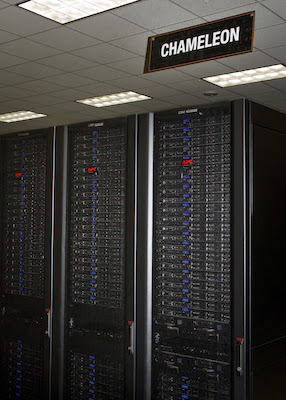
\includegraphics[width=0.5\columnwidth]{images/chameleon/Chameleon2.jpeg}
\caption{Chameleon Cloud Racks}
\end{figure}

\subsection{Network}\label{network}

Networking is changing rapidly, and the network fabric is as much a part
of the research focus of Chameleon as the compute or storage. For the
Chameleon network, every switch in the research network is a fully
OpenFlow compliant programmable Dell S6000-ON switch. Each node connects
to this network at 10 Gbps, and each unit~uplinks with 40Gbps per rack
to the Chameleon core network. The core switches (Dell S6000-ON) are
connected by~40 Gbps Ethernet links, which connect to the backbone
100Gbps services at both UC and TACC.~A Fourteen Data Rate (FDR)
Infiniband network (56Gbps) is also deployed on one SCU to allow
exploration of alternate networks.


\subsection{Shared Storage}\label{shared-storage}

While storage is dynamically provisioned to researchers to be used as an
experiment needs within the SCUs, Chameleon also provides a shared
storage system. The shared storage provides more than 3.6PB of raw disk
in the initial configuration, which is partitioned between a file system
and an object store that is persistent between experiments. The shared
storage is comprised of four Dell R630 servers with 128 GiB of RAM, four
MD3260 external drive arrays, and six MD3060e drive expansion chassis,
populated by 600 6TB near line SAS drives. The system also includes a
dozen PowerEdge R630 servers as management nodes to provide for login
access to the resource, data staging, system monitoring, and hosting
various OpenStack services.


\subsection{Heterogeneous Compute
Hardware}\label{heterogeneous-compute-hardware}

The heterogeneous hardware includes various technologies: GPU and FPGA
accelerators, SSD and NVMe storage, low-power ARM, Atom, and Xeon
systems-on-a-chip. With the exception of the low-power
systems-on-a-chip, each of the additional nodes is a Dell PowerEdge R730
server with the same CPUs as the R630 servers in our SCUs.

The two storage hierarchy nodes have been designed to enable experiments
using multiple layers of caching: they are configured with 512 GiB of
memory, two Intel P3700 NVMe of 2~TB each, four Intel S3610 SSDs of 1.6
TB each, and four 15K SAS HDDs of 600 GB each.

The GPU offering consists of two K80 GPU nodes, two M40 GPU nodes,
sixteen P100 GPU nodes. These nodes target experiments using
accelerators to improve the performance of some algorithms, experiments
with new visualization systems, and deep machine learning. Each K80 GPU
node is upgraded with an NVIDIA Tesla K80 accelerator, consisting of two
GK210 chips with 2496 cores each (4992 cores in total) and 24 GiB of
GDDR5 memory. Each M40 node is upgraded with an NVIDIA Tesla M40
accelerator, consisting of a GM200 chip with 3072 cores and 12 GiB of
GDDR5 memory. The P100 nodes have two GPU cards installed each,
providing 32 P100 GPUs in total. The P100 GPUs utilize GP100 chips
providing 3584 cores, with 16 GiB GDDR5 RAM in each card.~In order to
make it easy for users to get started with the GPU nodes, we have
developed a~\href{https://www.chameleoncloud.org/appliances/21/}{CUDA
appliance} that includes NVIDIA drivers as well as the CUDA framework.

\begin{longtable}[]{@{}llllll@{}}
\toprule
GPU & Chip & Cores per GPU & RAM per GPU & GPU per node & \# of
nodes\tabularnewline
Tesla K80 & GK 210 & 2496 $\times$ 2 & 24 GiB GDDR5 & 1 & 2\tabularnewline
Tesla M40 & GM 200 & 3072 & 12 GiB GDDR5 & 1 & 2\tabularnewline
Tesla P100 & GP100 & 3584 & 16 GiB GDDR5 & 2 & 16\tabularnewline
\bottomrule
\end{longtable}

The four FPGA nodes have a~Nallatech 385A board with an Altera Arria 10
1150 GX FPGA (up to 1.5 TFlops), 8 GiB DDR3 on-card memory, and dual
QSFP 10/40 GbE support. The Chameleon
\href{https://www.chameleoncloud.org/docs/bare-metal-user-guide/fpga/}{FPGA
User Guide}~provides details for conducting experiments on this
hardware.

The low-power systems are comprised of 8 low power Xeon servers (HP
ProLiant m710p with one 4-core Intel Xeon E3-1284L v4 processor), 8 Atom
servers (HP ProLiant m300 with one 8-core Intel Avoton-based System on a
Chip), and 24 ARM servers (HP ProLiant m400 with one 8-core AppliedMicro
X-gene System on a Chip). These are all delivered in a single HP
Moonshot 1500 chassis.

For more information on how you can reserve these nodes, see the
\href{https://www.chameleoncloud.org/docs/bare-metal-user-guide/\#heterogeneous_hardware}{heterogeneous
hardware section} of the bare metal user's guide.


\subsection{Live updates}
You can browse detailed information about the resources
offered~for bare metal reconfiguration in our
\href{https://www.chameleoncloud.org/user/discovery/}{Resource Discovery
Portal}.


\chapter{Getting Started}
\label{C:cc-start}

\FILENAME

We describe how you can get access to chameleon cloud under the
assumption that you are a student or a researcher that joins an
existing project on Chameleon cloud. You will need to follow the
following steps:

\section*{Step 1: Create~a Chameleon~account}

To get started using Chameleon you will need to
\href{https://www.chameleoncloud.org/register}{create a user account}.

You will be asked to agree to the
\href{https://www.chameleoncloud.org/terms/view/chameleon-user-terms/}{Chameleon
  terms and conditions} which, among others, ask you to acknowledge
the use of Chameleon in your publications. 

Acknowledgement of support from the Chameleon project and the
National Science Foundation should appear in any publication of
material, whether copyrighted or not, that describes work which
benefited from access to Chameleon cyberinfrastructure resources. The
suggested acknowledgement is as follows: ``Results presented in this
paper were obtained using the Chameleon testbed supported by the
National Science Foundation''.

\begin{IU}
  As part of creating an account you may request PI status. However
  you are not a PI as you will be joining a project.
\end{IU}

\section*{Step 2: Create or join a project}

To use Chameleon, you will need to be associated with a
\href{https://www.chameleoncloud.org/docs/user-faq/\#toc-how-do-i-apply-for-a-chameleon-project-}{project}
that is assigned an
\href{https://www.chameleoncloud.org/docs/user-faq/\#toc-what-are-the-project-allocation-sizes-and-limits-}{allocation}.
This means that you either need to

\begin{enumerate}

\item \textbf{\href{https://www.chameleoncloud.org/user/projects/new/}{apply
for a new project}} or 

\item
\textbf{\href{https://www.chameleoncloud.org/docs/user-faq/\#toc-my-pi-professor-colleague-already-has-a-chameleon-project-how-do-i-get-added-as-a-user-on-the-project-}{ask
the PI of an existing Chameleon project to add you}.}

\end{enumerate}

A project is headed by a project PI, typically
\href{https://www.chameleoncloud.org/docs/user-faq/\#toc-who-is-eligible-to-be-chameleon-pi-and-how-do-i-make-sure-that-my-pi-status-is-reflected-in-my-profile-}{a
faculty member or researcher scientist at a scientific institution}. If
you are a student we recommend that you ask your professor to work with
you on creating a project. Please note that you must not create a
project by yourself and that you indeed need to work with your
professor. 

In case you need to do a project application typically consists of
about one paragraph description of the intended research and takes one
business day to process.

Enrolling you into an existing research or class project depends on
the time availability of the project lead or professor of your
class. It is important that you communicate your chameleon cloud
account name to the project lead so they can easily add you. Make sure
you really give them only your chameleon account name and potentially
your organizational e-mail, Firstname, and Lastname so they can check
you are eligible to get access. 

\begin{IU}
Indiana University students that take the e516 and e616 classes will
have to fill out a google form in which they communicate the chameleon
cloud name. You can already apply for an account name, but do not
apply for a project. If you nevertheless apply for a project, we will
hear from the administrators and you will receive a point deduction.
\end{IU}

\section*{Step 3: Start using Chameleon!}\label{using-chameleon}

Now that you have enrolled and once you are added to the project by your
project lead you can start using chameleon cloud. However be reminded
that you ought to shut down the resources/VMs whenever they are not in
use to avoid unnecessary charging. Remember the project has imited
time on chameleon and any unused time will be charged against the project.

Chameleon provides two types of resources with links to their respective
users guides below:

\textbf{\href{https://www.chameleoncloud.org/docs/bare-metal-user-guide-old/}{Bare
Metal User Guide}} will tell you how to use Chameleon bare metal
resources which provide strong isolation and allow you maximum control
(reboot to new operating system, reboot the kernel, etc.)

\textbf{\href{https://www.chameleoncloud.org/docs/user-guides/openstack-kvm-user-guide/}{OpenStack
KVM User Guide}} will tell you how to get started with Chameleon's
OpenStack KVM cloud which is a multi-tenant environment providing weak
performance isolation. 

If you have any questions or encounter any problems, you can check out
our \href{https://www.chameleoncloud.org/docs/user-faq/}{User FAQ},
or \href{https://www.chameleoncloud.org/user/help/}{submit a ticket}.

\begin{IU}
As part of the classes you will need to first pass a cloud {\em security}
drivers licence test.  The test is designed so that you think about
gaining access to a VM securely and how to properly secure the
VM. Once passed, access is typically provided by midterm time. You are
not allowed to constantly run VM's and must shut them down if not in
use. You will get point deductions if we detect you do not obey by
this rule. We have access to log files about your VM usage.
\end{IU}


\section{Charge Rates}
\label{C:cc-charge}

It is important to fully understand the charge rates of your VM and storage use.

Chameleon has two types of limitations, introduced to promote fair resource
usage to all:

\begin{description}

\item  [Allocation:] Chameleon projects are limited to a per-project allocation
  currently set to~20,000 service units for 6 months. Allocations can be
  renewed or extended (see
  \href{index.html\#toc-project-and-allocation-management}{Project and
  Allocation Management} section for more details on Chameleon
allocations.)

  \item [Lease:] To ensure fairness to all users, resource reservations (leases)
  are limited to a duration of 7 days. However, an active lease within
  48 hours of its end time can be prolonged by up to 7 days from the
  moment of request if resources are available. To prolong a lease,
  click on the ``Update Lease'' button in the Reservations panel of the
  CHI OpenStack dashboard, and enter the additional duration requested
  in the ``Prolong for'' box including the unit suffix, e.g. ``5d'' for
  5 days or ``30m'' for 30 minutes. If there is an advance reservation
  blocking your lease prolongation that could potentially be moved,
  you can interact through the users mailing list to coordinate with
  others  users.~Additionally, if you know from the start that your
  lease will  require longer than a week and can justify it, you can
  \href{https://www.chameleoncloud.org/user/help/ticket/new/}{contact
    Chameleon staff via the ticketing system} to request a one-time
  exception to create a longer lease. The lease must be requested by
  the PI.

\end{description}

\subsection{Service Units}

Chameleon allocations can consist of several components of the system.
Users can request allocation of individual compute nodes, storage
servers, or complete Scalable Compute Units (SCUs) which contain compute
servers, storage nodes, and an open flow switch.

Compute servers are allocated in Service Units (SUs), which equates to
one hour of wall clock time on a single server (for virtual machines, an
SU is 24 cores with up to 128GB of RAM). Note this unit differs from
traditional HPC or cloud service units that are charged in core-hours; a
Chameleon SU is a full server, as the type of experiments and
performance measurements users may wish to do may be contaminated by
sharing nodes.

Storage servers are also charged in SUs, at 2x the rate of compute
servers (i.e., 1 hour allocation of 1 storage server == 2 SUs). SCUs are
charged at the rate of 50 SUs per wall clock hour (42 compute servers, 4
storage nodes, plus one OpenFlow switch).

An allocation may make use of multiple SCUs, up to the size of the full
testbed.

For example, a user wishing to provision a 10 node cluster +1 storage
server for a 1 week experiment should budget
\texttt{{[}(10\ +\ 2)\ SUs\ per\ hour{]}\ *\ {[}7\ days\ *\ 24\ hours/day{]}\ =\ 2,016\ SUs}
for that experiment.

SUs are charged the same regardless of use case. Hence, whether asking
for bare metal access, virtual machine access, or use of default images,
the charge is the same --- you are charged for the fraction of the
resource your experiment occupies, regardless of the type of the
experiment.

The basic principle for charging service units for Chameleon resources
is to evaluate the amount of time a fraction of the resource is
unavailable to other users. If a reservation is made through the portal
for a particular date/time in the future, the user will be charged for
this time regardless of whether the reservation is actually used, as the
Chameleon scheduling system will have to drain the appropriate part of
the system to satisfy the reservation, even if the nodes requested are
not actually used. A reservation request may be cancelled in which case
no charges will apply.

\subsection{Project Allocation Size}

CUrrently Chameleon is operating on a ``soft allocation
model'' where each project, if approved, will receive a startup
allocation of 20,000 SUs for six months that can be both recharged
(i.e., more SUs can be added) and renewed (i.e., the duration can be
extended) via submitting a renew/recharge request. This startup
allocation value has been designed to respond to both PI needs (i.e.,
cover an amount of experimentation needed to obtain a significant
result) and balance fairness to other users (it represents roughly 1\%
of testbed six months' capacity). Requests for these startup projects
will receive a fast track internal review (i.e., users can expect them
to be approved within a few days).

A PI can apply for multiple projects/allocations; however, the number of
held allocations will be taken into account during review.

As our understanding of user need grows we expect the Chameleon
allocation model to evolve towards closer reflection of those needs in
the form of more differentiated allocations that will allow us to give
larger allocations to users for longer time.

\begin{IU}
  Please be mindful to shutting down your VMS when not in use as even VMs 
  that do not do any calculations get charged. In past classes we had students 
  that did not shut down their VMs and within 2 weeks used up all SUs 
  for the entire class of 70 students. We like to avoid this. In future cases 
  we will assign the grade ``F'' to such students, as is customary also 
  in other universities.
\end{IU}


\section{OpenStack Virtual Machines}
\label{C:cc-guide}

\FILENAME\

OpenStack is an Infrastructure as a Service (IaaS) platform that allows
you to create and manage virtual environments. Chameleon provides an
installation of OpenStack version 2015.1~(Kilo)~using the~KVM
virtualization technology.

Since the KVM hypervisor is used on this cloud, any virtual machines you
upload must be compatible with KVM.

This tutorial provide basic information about how to use the OpenStack
web interface and provides some information specific to using OpenStack
KVM on Chameleon.

\subsection{Web Interface}\label{web-interface-horizon}

An easy way to use OpenStack KVM on Chameleon~is via
the~\href{https://openstack.tacc.chameleoncloud.org/dashboard}{OpenStack
  web interface} also known as Horizon. You log into the web interface
using your Chameleon username and password. If you change your
Chameleon password in the portal, that change will propagate to the
OpenStack KVM interface~in about 5 minutes.

The initial log in page appears as:

\begin{center}
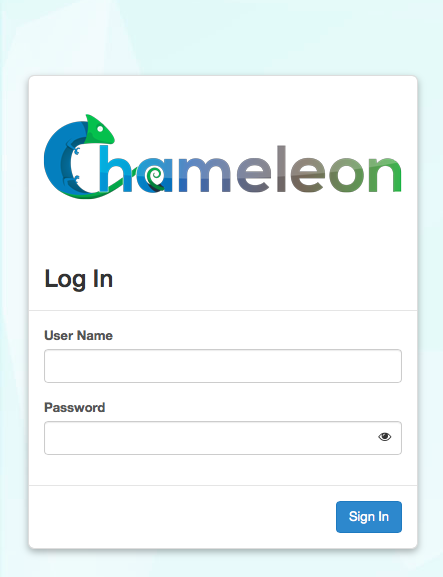
\includegraphics[width=0.3\columnwidth]{images/chameleon/chameleon-login.png}
\end{center}

After a successful log in, you will see the Overview page as shown
below. This page provides a summary of your current and recent usage and
provides links to various other pages. Most of the tasks you will
perform are done via the menu on the lower left and will be described
below. One thing to note is that on the left, your current project is
displayed. If you have multiple Chameleon projects, you can change which
of them is your current project. All of the information displayed and
actions that you take apply to your current project. So in the screen
shot below, the quota and usage apply to the current project you have
selected and no information about your other projects is shown.

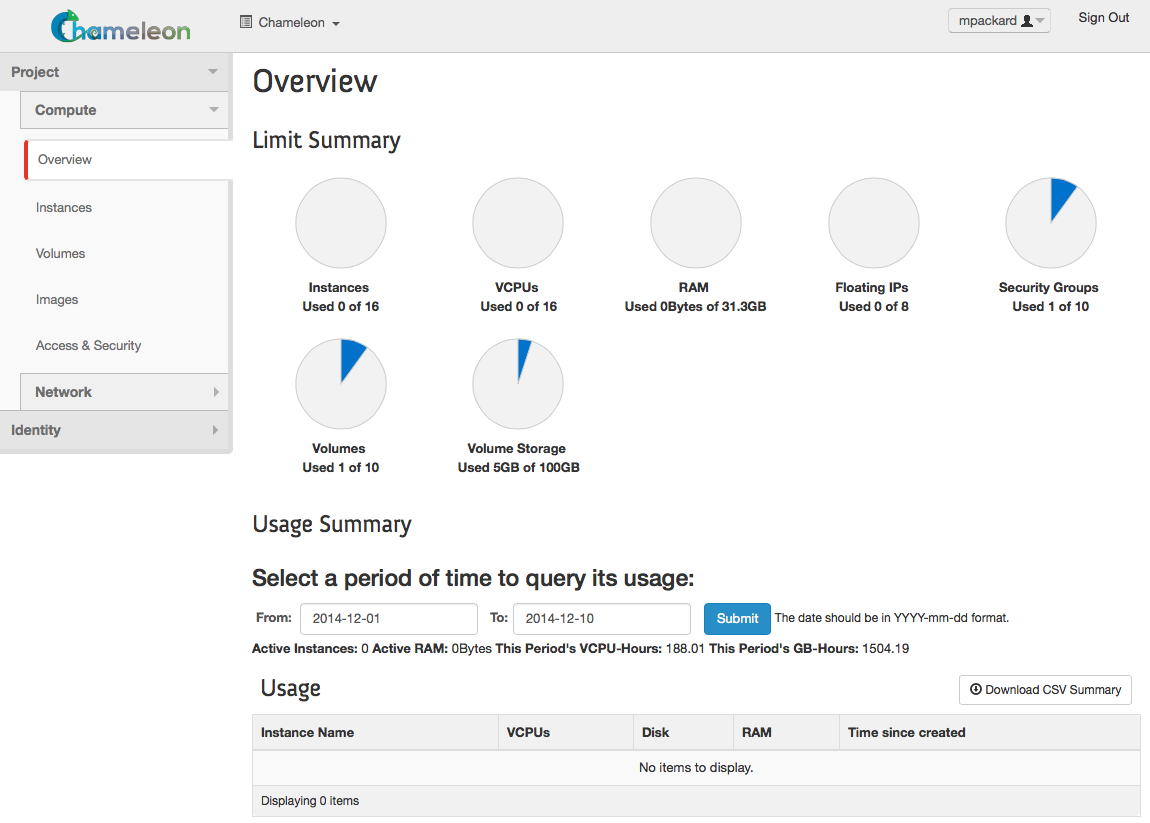
\includegraphics[width=0.8\columnwidth]{images/chameleon/openstack_alamo_overview.png}

\subsubsection{Managing Virtual Machine Instances}\label{managing-virtual-machine-instances}

One of the main activities you'll be performing in this web interface is
the management of virtual machines, or instances. You do this via the
Instances page that is reachable from the menu in the lower left of the
Overview page. An example Instances page is shown below. For instances
that you have running, you can click on the name of the instance to get
more information about it and to access the VNC interface to the
console. The dropdown menu to the left of the instance lets you perform
a variety of tasks such as suspending, terminating, or rebooting the
instance.

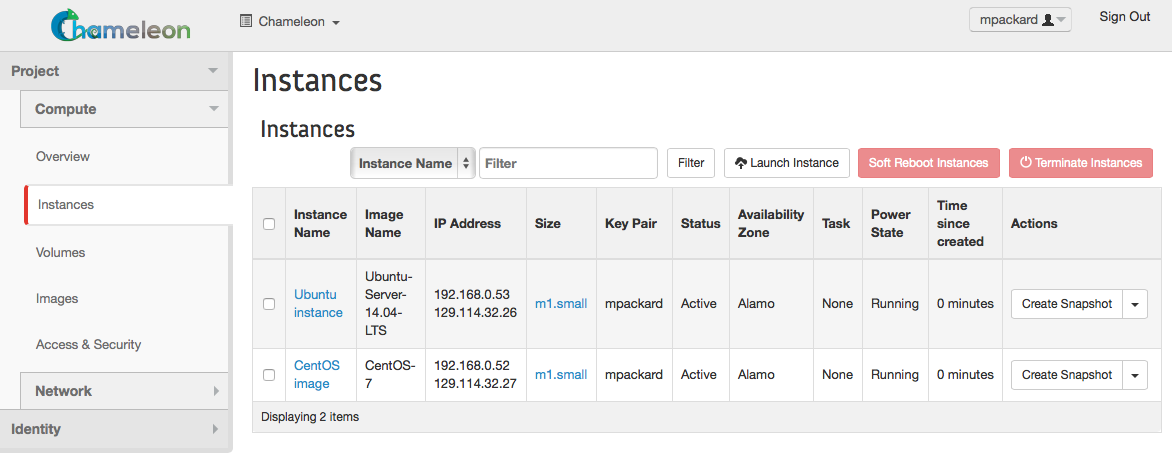
\includegraphics[width=0.8\columnwidth]{images/chameleon/openstack_alamo_instances.png}

The Instances page also lets you create new virtual machines by using
the `Launch Instance' button in the upper-right. When you click this
button, a dialog window pops up. In the first `Details' tab, you select
the `Instance Boot Source' of the instance, which is either an `Image',
a `Snapshot' (an image created from a running virtual machine), or a
`Volume' (a persistent virtual disk that can be attached to a virtual
machine). If you select `Boot from image', the Image Name dropdown
presents a list of virtual machine images that we have provided, that
other Chameleon users have uploaded and made public, or images that you
have uploaded for yourself. If you select `Boot from snapshot', the
Instance Snapshot dropdown presents a list of virtual machine images
that you have created from your running virtual machines.

On the Details tab, you also provide a name for this instance (to help
you identify instances that you are running), and select the amount of
resources (Flavor) to allocate to the instance. If you select different
flavors from the Flavor dropdown, their characteristics are displayed on
the right.

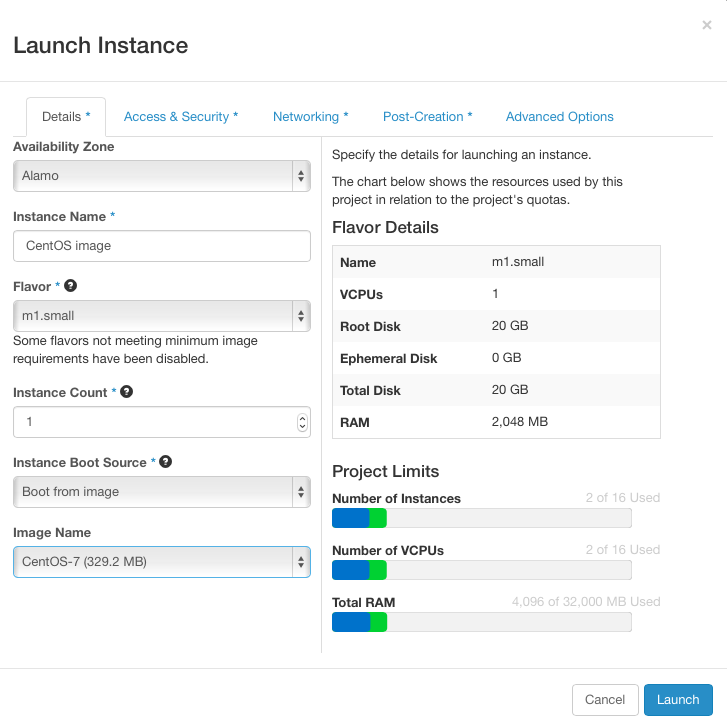
\includegraphics[width=0.8\columnwidth]{images/chameleon/openstack_alamo_launch_details.png}

The next tab is `Access \& Security', where you select an SSH keypair
that will be inserted into your virtual machine. These keypairs can be
uploaded via the main `Access \& Security' section. You will need to
select a keypair here to be able to access an instance created from one
of the public images Chameleon provides. These images are not configured
with a default root password and you will not be able to log in to them
without configuring an SSH key.

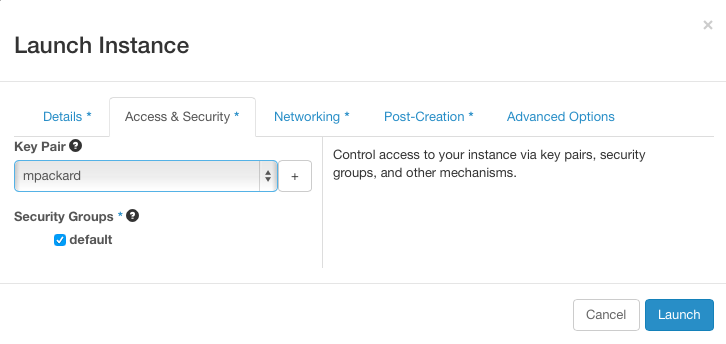
\includegraphics[width=0.8\columnwidth]{images/chameleon/openstack_alamo_launch_access.png}

Next is `Networking', where you select which network should be
associated with the instance. Click the + next to your your project's
private network (PROJECT\_NAME-net), not ext-net.

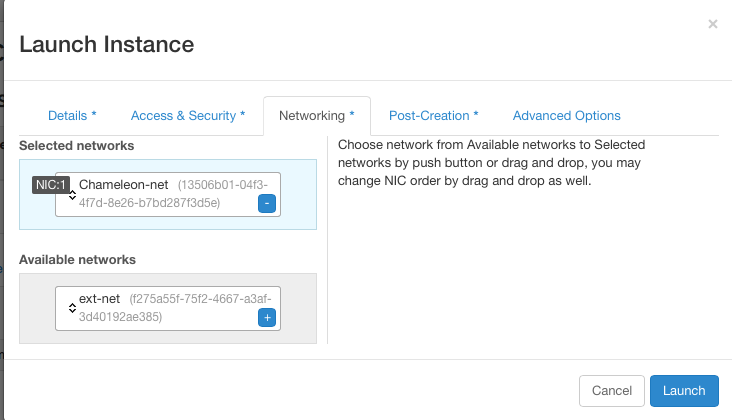
\includegraphics[width=0.8\columnwidth]{images/chameleon/openstack_alamo_networking.png}

Once you do this, you can Launch your instance and the Instances page
will show progress as it starts.

If you would like to assign a public IP address to your VM, you can do
that while it is booting up. Click on the dropdown under \emph{Actions}
and choose \emph{Associate Floating IP}. Choose an IP from the \emph{IP
Address} menu and click \emph{Associate}. If there are no addresses
available, click the + and follow the prompts to add one.

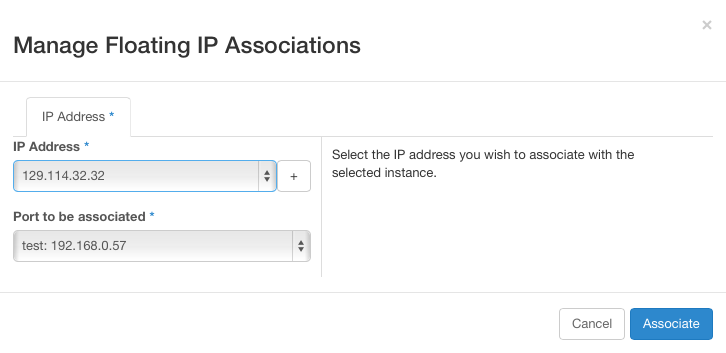
\includegraphics[width=0.8\columnwidth]{images/chameleon/openstack_alamo_floating.png}

OpenStack injects your SSH key into the VM and you can use the
corresponding private SSH key to log in to the VM. You will need to use
the public IP assigned to your VM to connect from outside of Chameleon,
or connect through an existing instance that both a public and private
IP.

\textbf{Note that the images we provide do not allow SSH into the root
account. For root access, SSH into the instance as user `cc' and then
use the \emph{sudo} command to become root.}

We have enabled auto-login for the cc user on the console of our
supported images. This should aid in debugging if you are unable to
reach the instane via ssh for some reason.

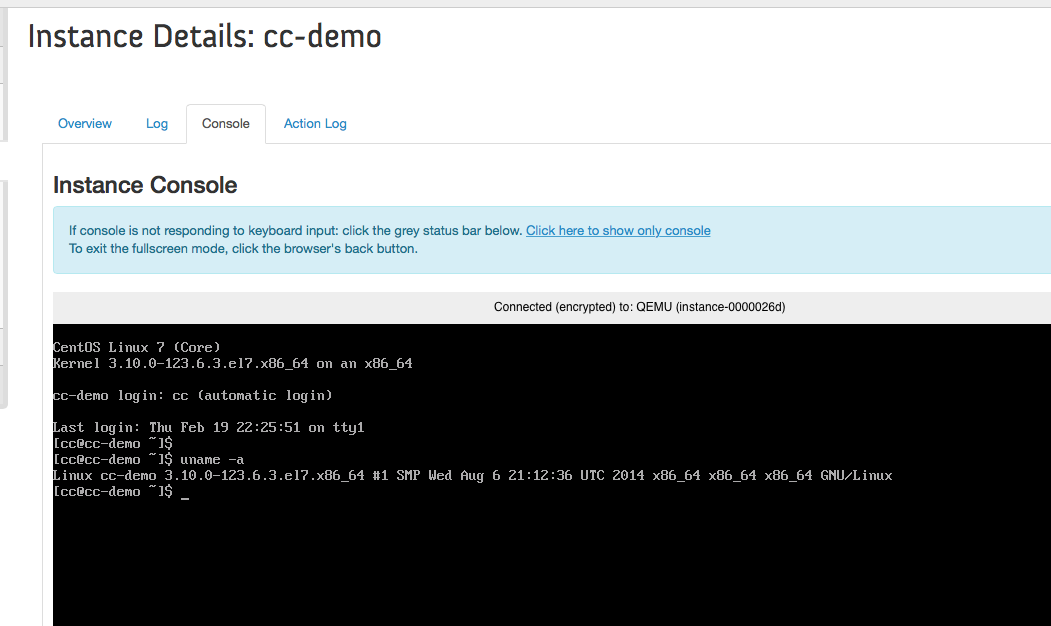
\includegraphics[width=0.8\columnwidth]{images/chameleon/openstack_alamo_console.png}

\subsubsection{Snapshots}\label{snapshots}

The instance list page shown above has an option `Create Snapshot' that
allows you to save a copy of the disk contents of a running virtual
machine. This allows you to start new virtual machines in the future
that are identical to this one and is an easy way to save any changes
you make to a running virtual machine.

\subsubsection{Firewall (Access Security)}\label{firewall-access-security}

Each project has control over their own firewall settings for their
instances. At minimum you'll probably want to allow SSH access so you
can reach your instances.

To enable this traffic, you need to configure the security group used by
your virtual machine. You can see a list of your security groups using
the ``Access \& Security'' link on the left.

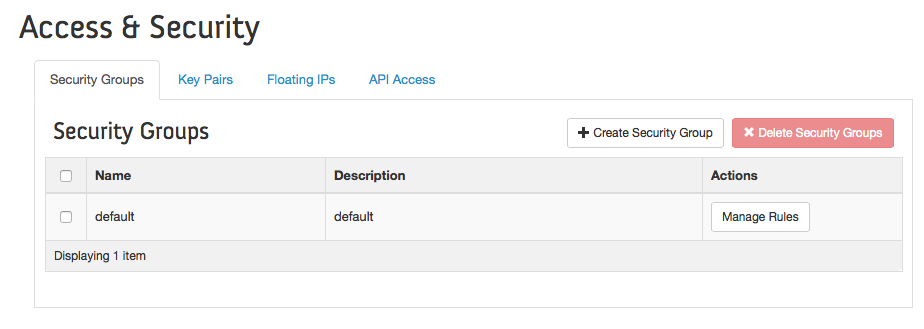
\includegraphics[width=0.8\columnwidth]{images/chameleon/openstack_alamo_security_groups.png}

To edit a security group, click on ``Edit Rules''. This opens a page
showing the existing rules in the security group.

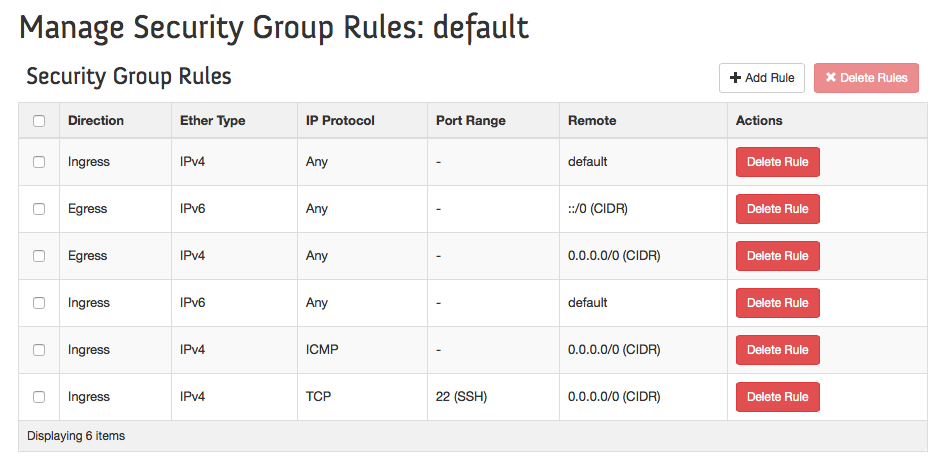
\includegraphics[width=0.8\columnwidth]{images/chameleon/openstack_alamo_edit_rules.png}

Click on ``Add Rule'' and choose the \emph{SSH} rule from the list, and
click \emph{Add}. Modifications are automatically propagated to the
OpenStack cloud. Feel free to add other rules as necessary.

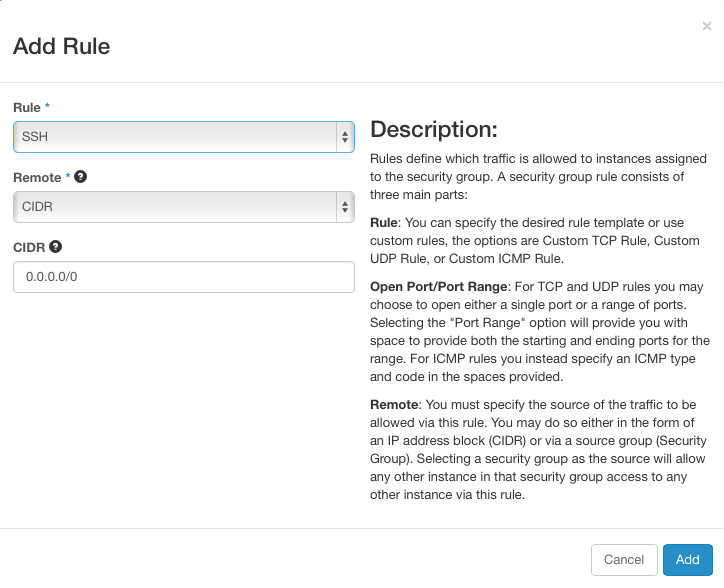
\includegraphics[width=0.8\columnwidth]{images/chameleon/openstack_alamo_add_secgroup_rule.png}

\subsection{OpenStack REST Interfaces}\label{openstack-rest-interfaces}

The OpenStack REST Interfaces are supported on Chameleon over secure
HTTP connections. You can download your OpenStack credentials file from
the web interface via the ``Access \& Security'' link in the left of any
page and then click on the ``API Access'' link on the top.

You can then install the OpenStack command line clients following
\href{http://docs.openstack.org/user-guide/common/cli_install_openstack_command_line_clients.html}{these
instructions}. If using pip, we recommend setting up a virtualenv.

The SSL certificate used by Chameleon~is trusted by most operating
systems, so you shouldn't have to provide any extra options to OpenStack
commands, i.e. ``nova list'' should work.~If your command-line tool
complains about the certificate,
\href{http://curl.haxx.se/docs/caextract.html}{download the Mozilla CA
bundle from the cURL website} and run the OpenStack client tools with
the --os-cacert cacert.pem arguments.

\begin{comment}

 
\subsection{EC2 Interface}\label{ec2-interface}

\begin{IU}
Last time we used the EC2 interface it was broken, thus we no longer
recommend using it
\end{IU}

OpenStack KVM on Chameleon~supports the EC2 interface for programmatic
access. You can download your EC2 credentials from the web interface via
the ``Access \& Security'' link in the left of any page and then click
on the ``API Access'' link on the top. You should see a `Download EC2
Credentials' button on the top-right. Note that you have different EC2
credentials for each Chameleon project you participate in. If you are a
member of multiple Chameleon projects, we request that you use the
corresponding EC2 credentials when starting virtual machines for a
project.

\end{comment}

\subsection{Downloading and uploading data}\label{downloading-and-uploading-data}

You can use the OpenStack command line clients to download data from and
upload data to Chameleon clouds. Configure your environment by following
the ``OpenStack REST Interfaces'' section above, then use the following
commands:

\begin{itemize}
\item
  \verb|glance image-download| to download images and snapshots from
  Glance
\item
  \verb|glance\ image-create| to upload images and snapshots to Glance
\item
  \verb|cinder upload-to-image| to convert a Cinder volume to a
  Glance~image
\item
  \verb|cinder create [--image-id <image-id>] [--image <image>]|
  to create a Cinder volume from a Glance image
\end{itemize}



\FILENAME

\chapter{Horizon Graphical User Interface}

\section{Configure~resources}\label{configureresources}

Once your lease is started, you are almost ready to start an instance.
But first, you need to make sure that you will be able to connect to it
by setting up a key pair. This only has to be done once per user per
project.

Go to Project \textgreater{} Compute \textgreater{} Access \& Security,
then select the Key Pairs tab.

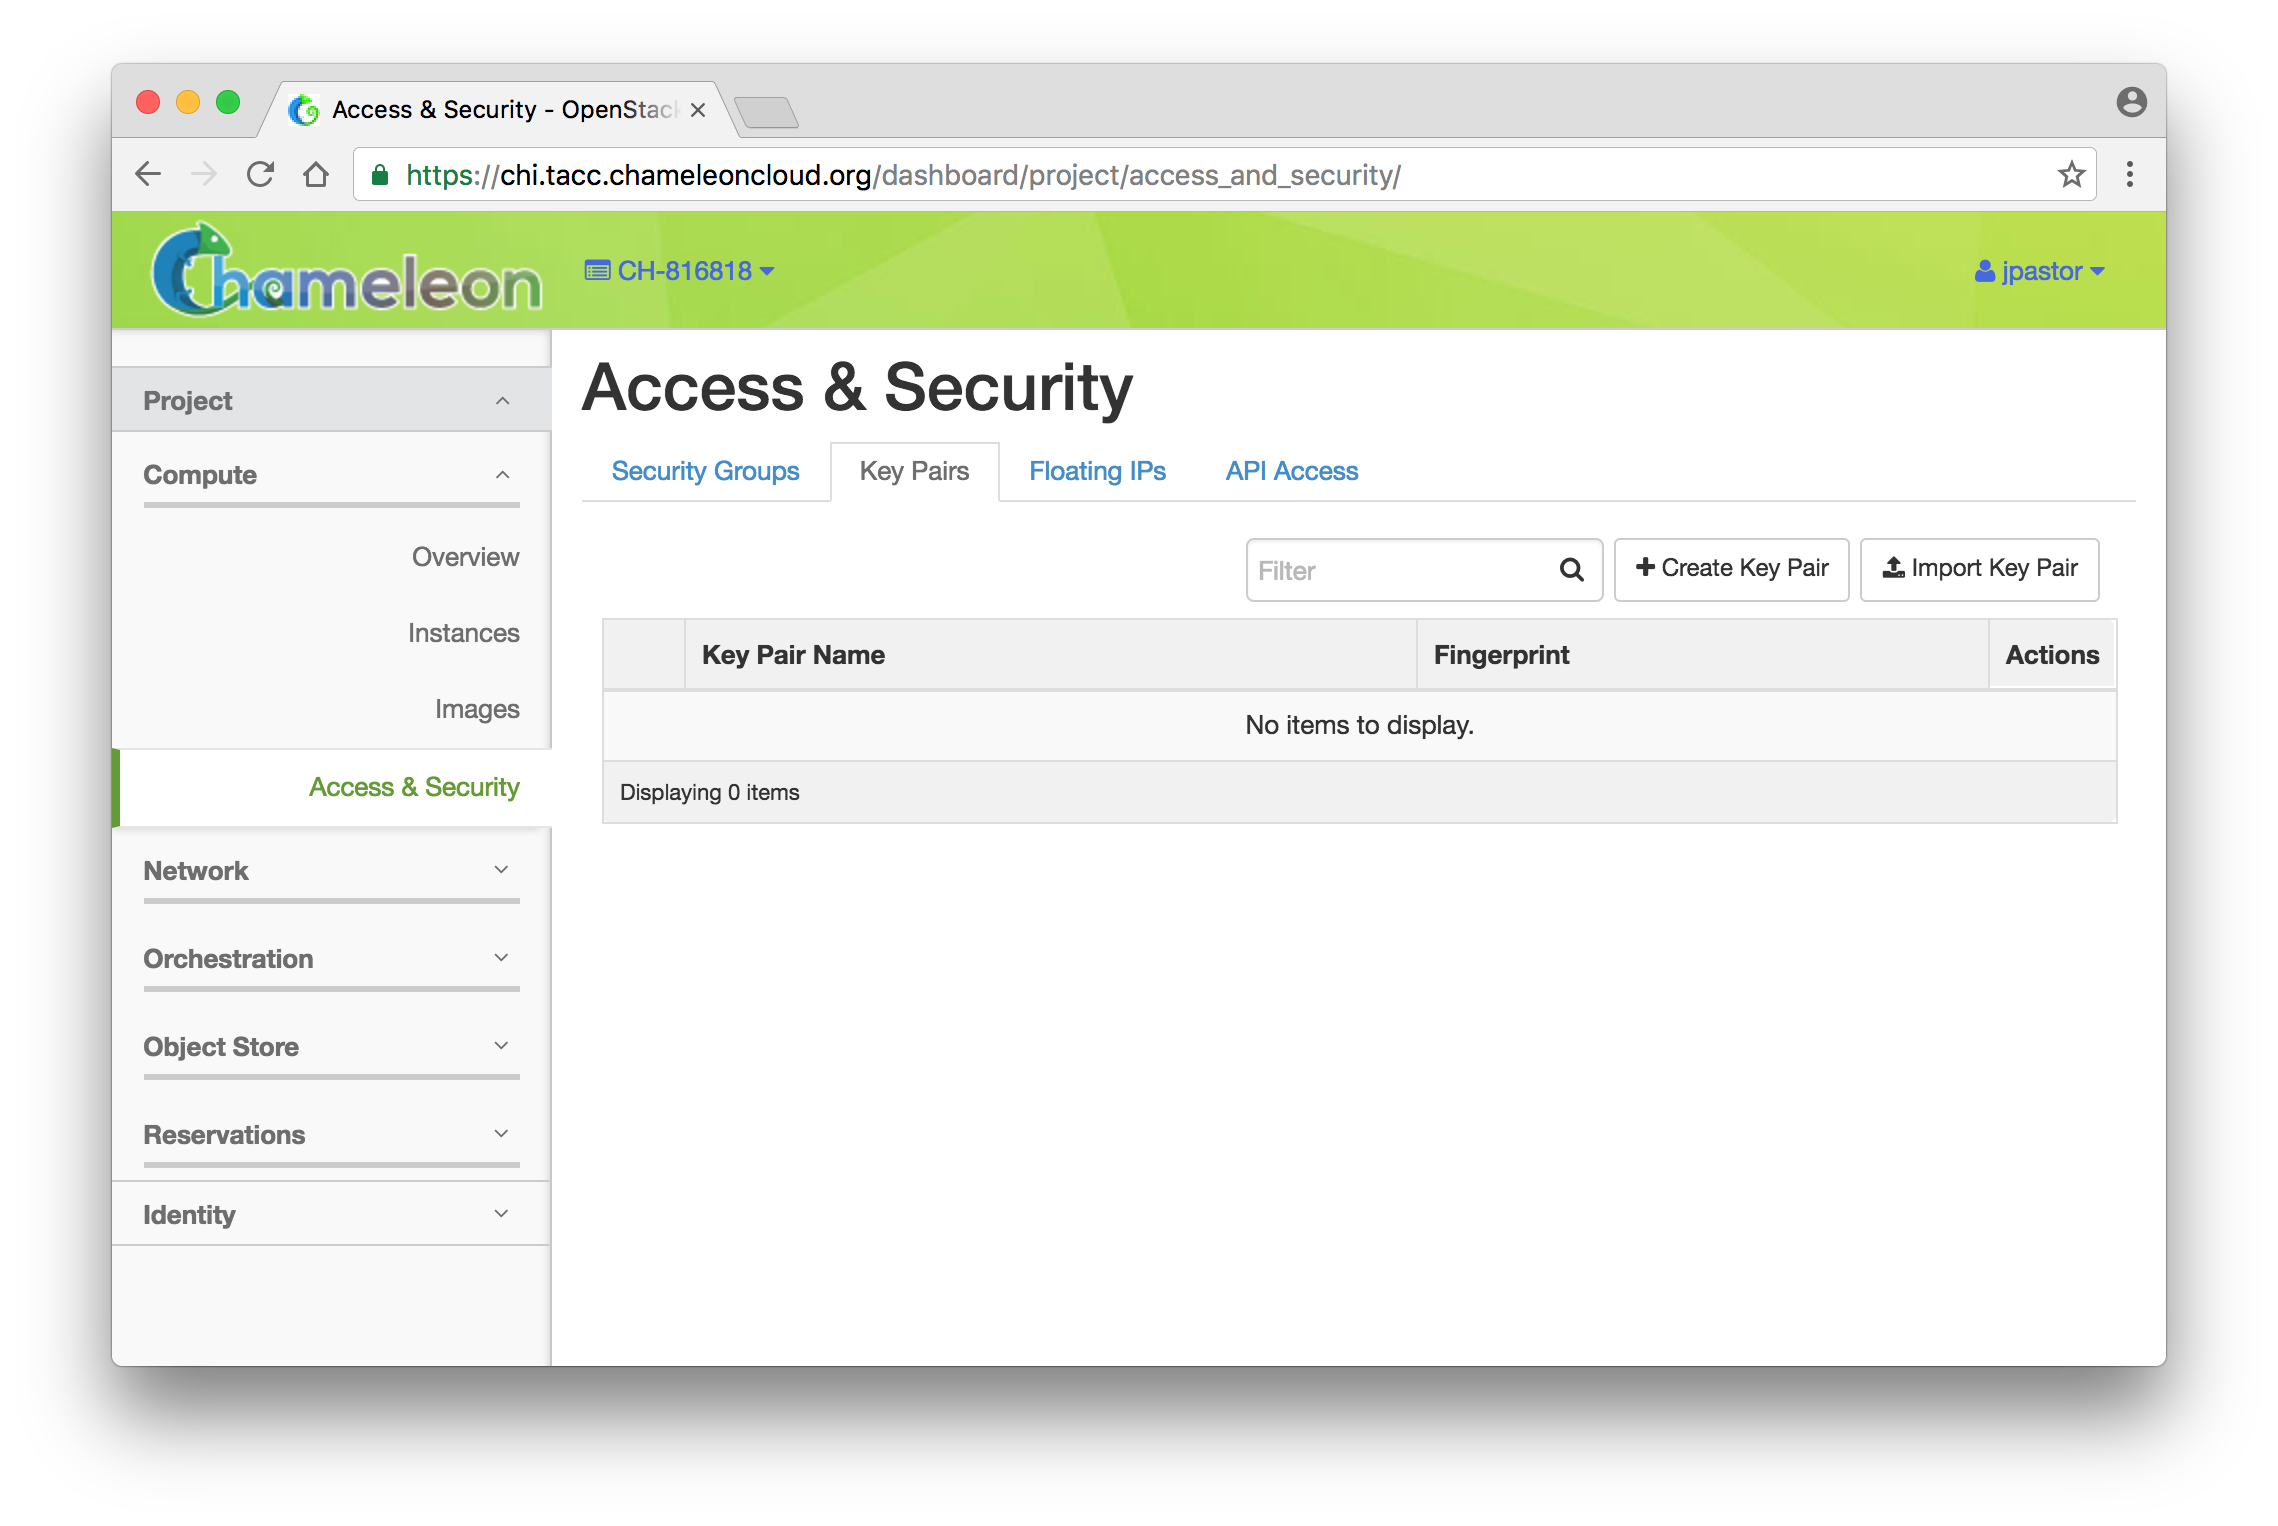
\includegraphics[width=\columnwidth]{images/chameleon/Screen-Shot-2016-10-26-at-14-37-00.png}

Here you can either ask OpenStack to create an SSH key pair for you (via
the ``Create Key'' Pair~button), or, if you already have an SSH key pair
on your machine and are happy to use it, click on ``Import Key Pair''.

If you chose to import a key pair, you will be asked to enter a name for
the key pair, for example laptop. In the ``Public Key'' box, copy the
content of your SSH public key. Typically it will be at
\textasciitilde{}/.ssh/id\_rsa.pub. On Mac OS X, you can run in a
terminal:
~\texttt{cat\ \textasciitilde{}/.ssh/id\_rsa.pub\ \textbar{}\ pbcopy}\\
It copies the content of the public key to your copy/paste buffer. Then
you can simply paste in the ``Public Key'' box.

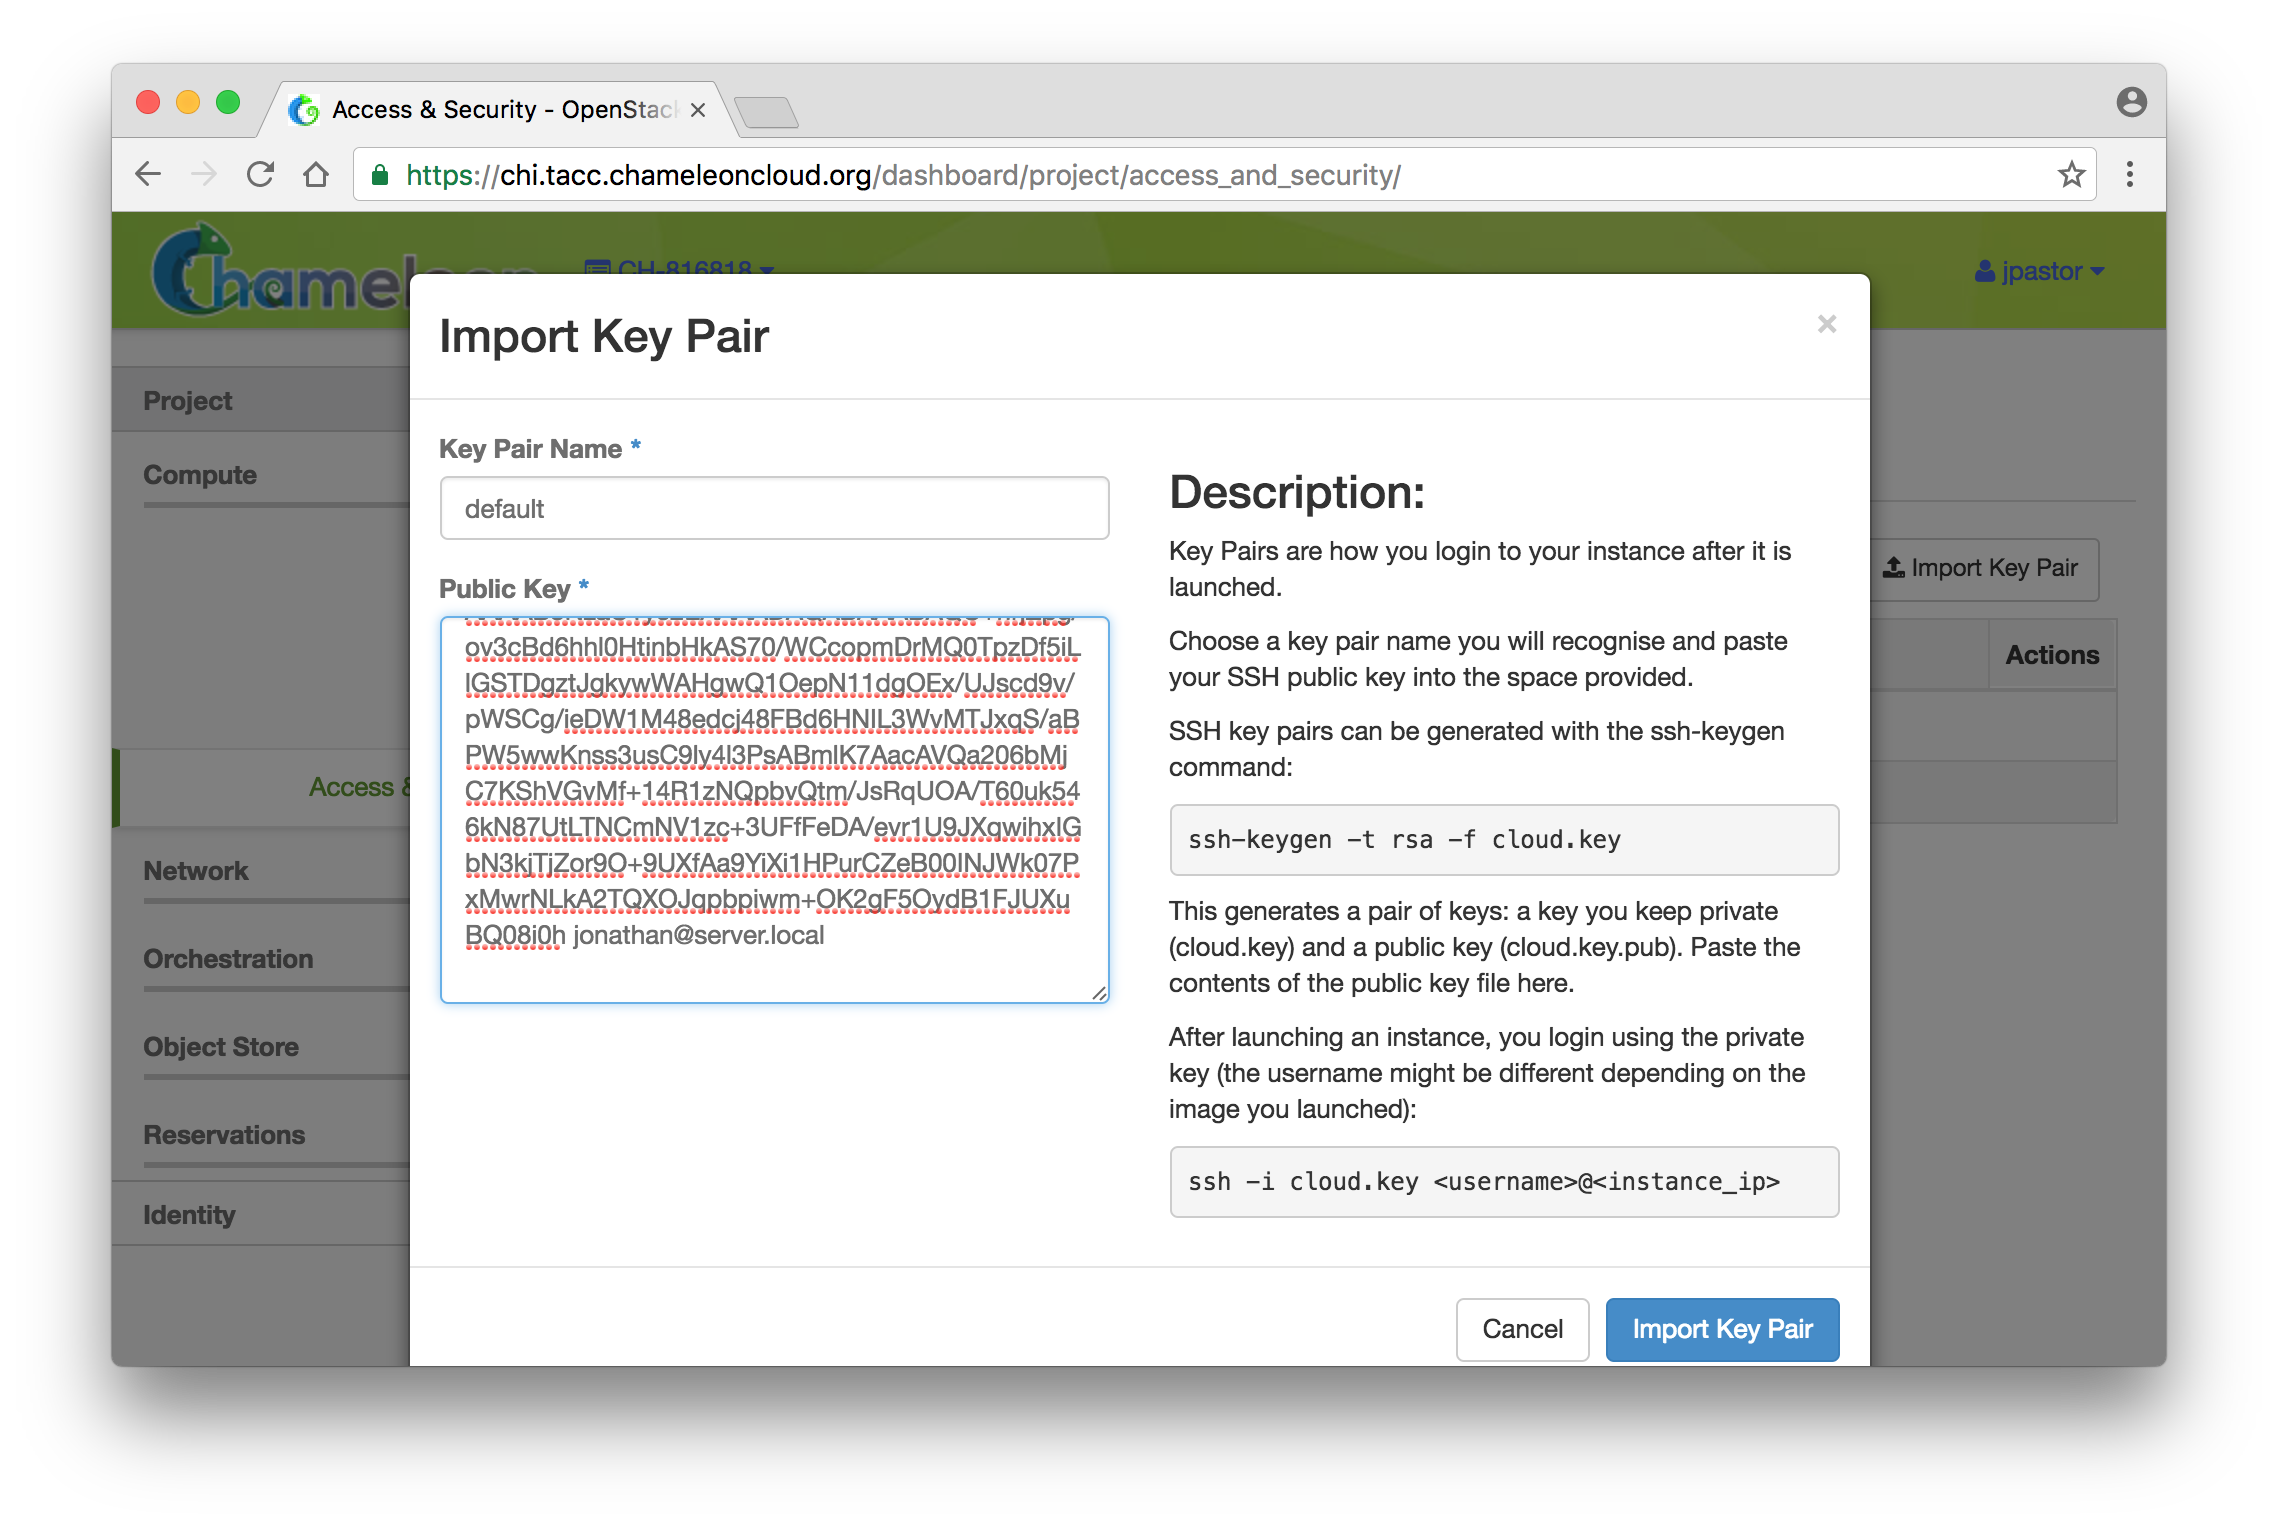
\includegraphics[width=\columnwidth]{images/chameleon/Screen-Shot-2016-10-26-at-14-37-18.png}

Then, click on the blue ``Import Key~Pair'' button. This should show you
the list of key pairs, with the one you just added.

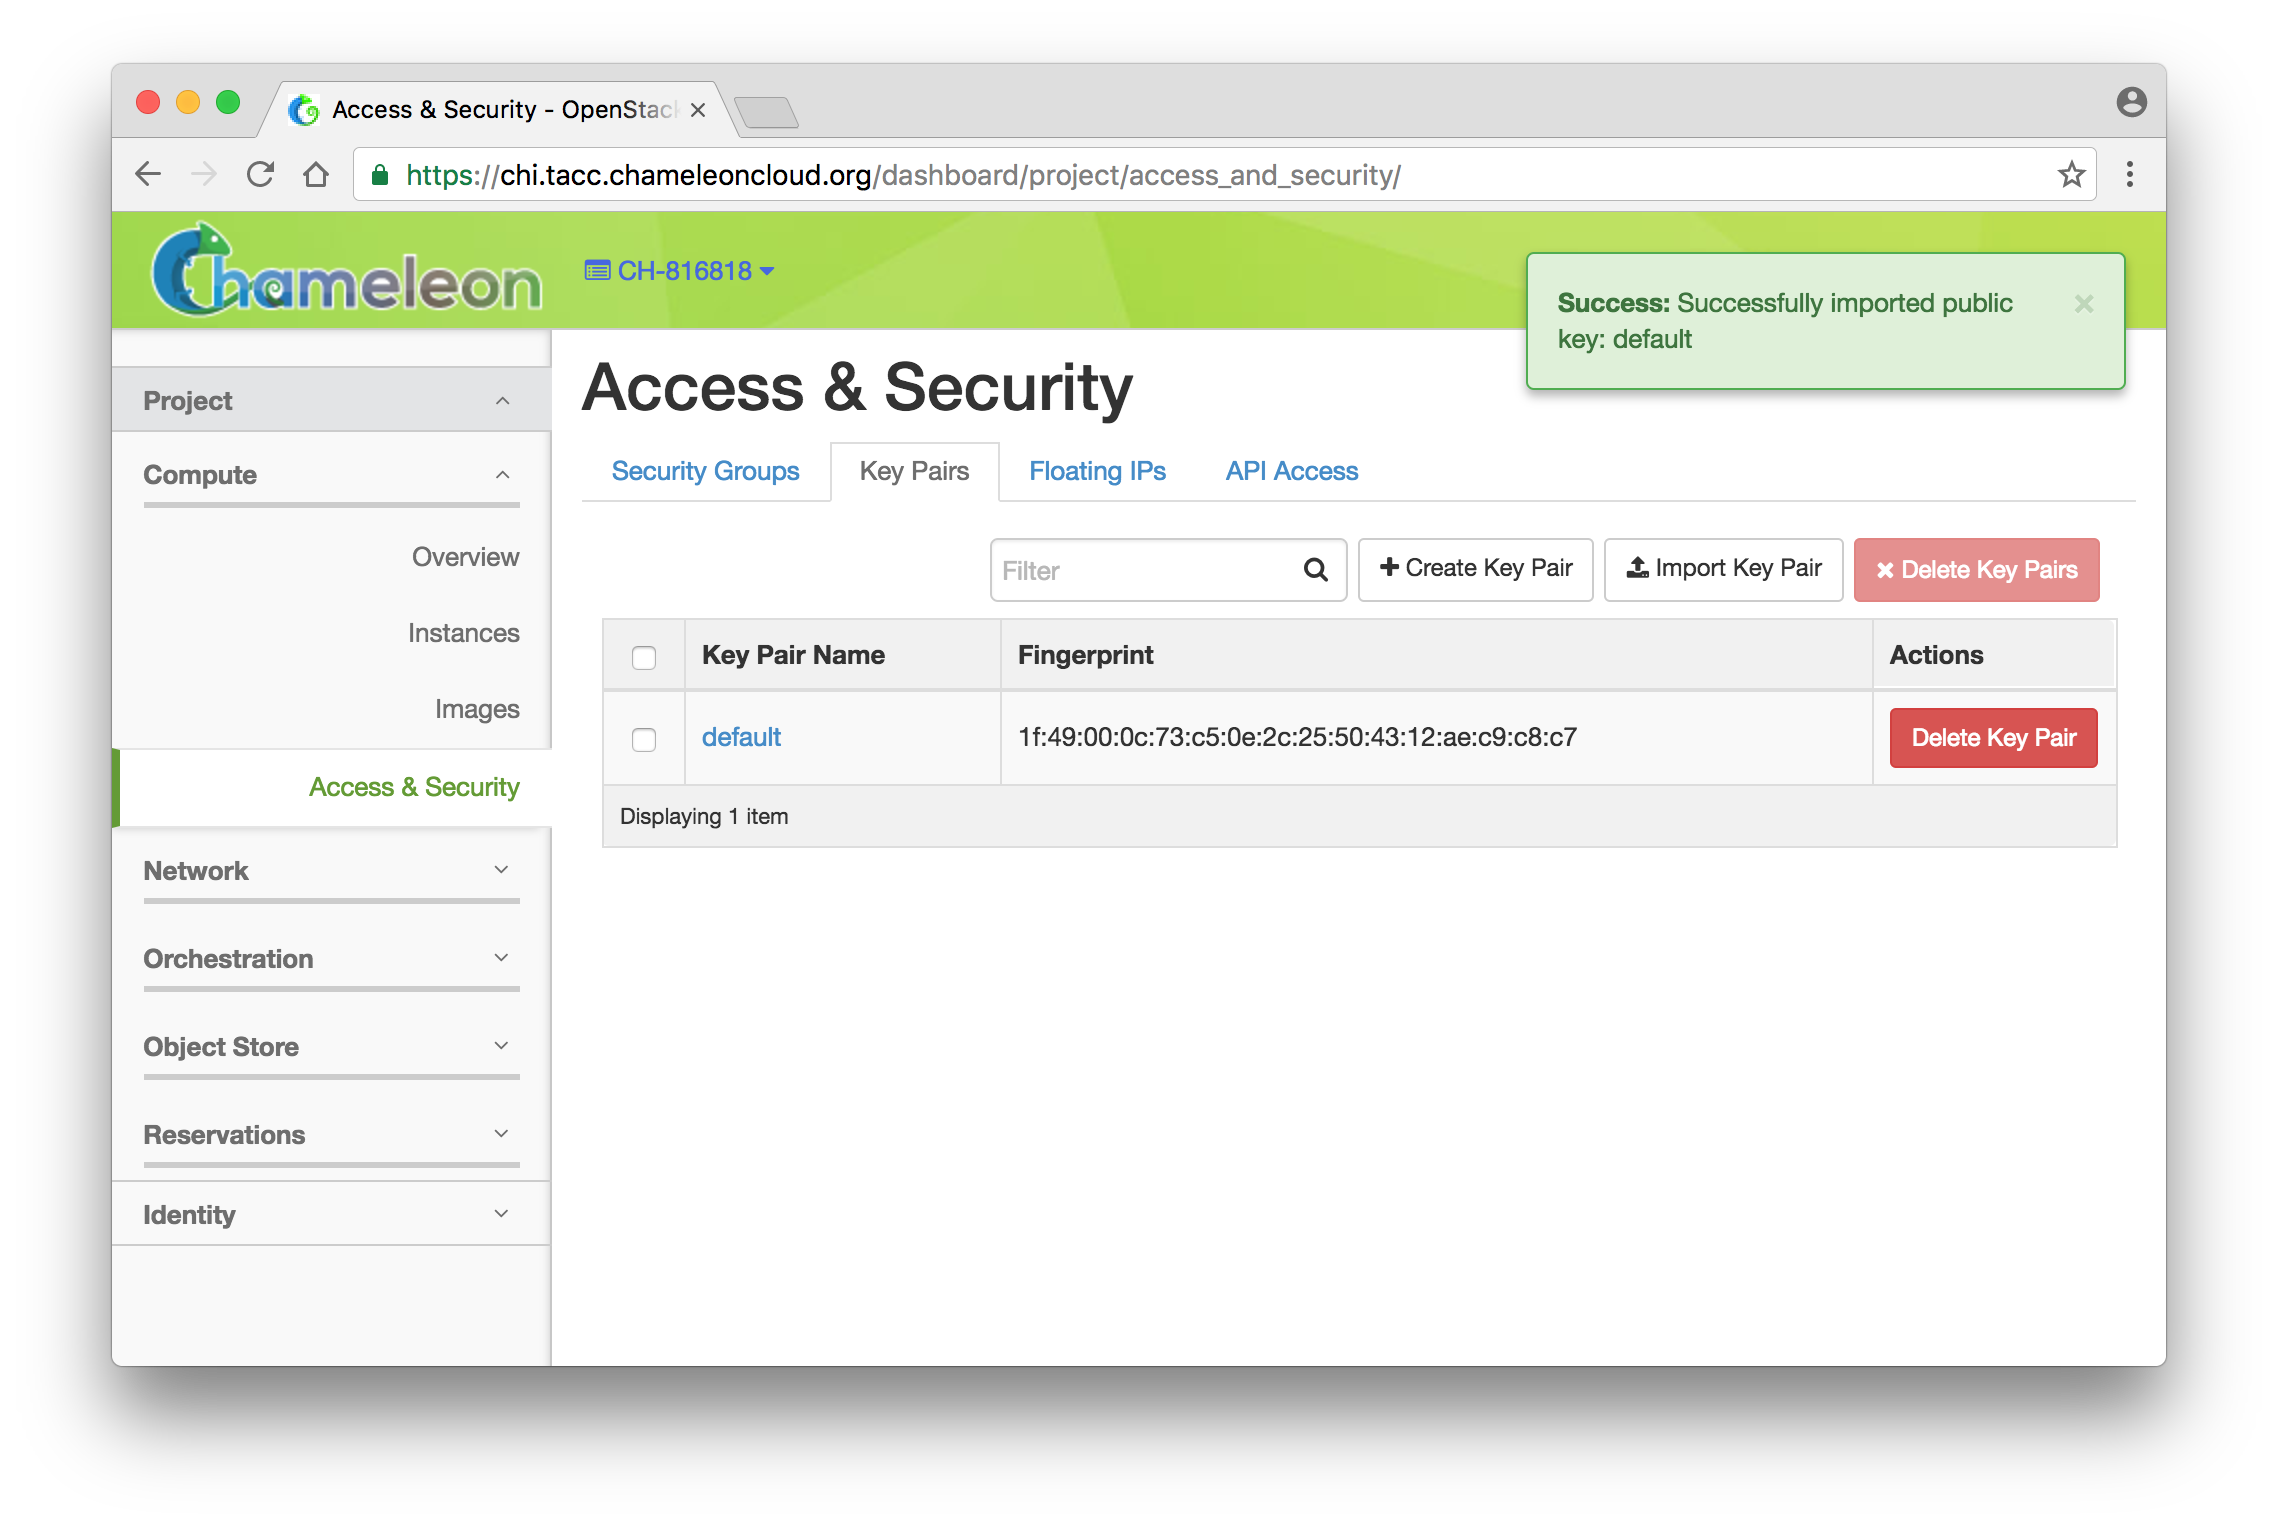
\includegraphics[width=\columnwidth]{images/chameleon/Screen-Shot-2016-10-26-at-14-37-52.png}

For those already familiar with OpenStack, note that Security Groups are
not functional on bare-metal. All instances ports are open to the
Internet and any security group rule you add will not be~respected.

~

Now, go to the ``Instances'' panel.

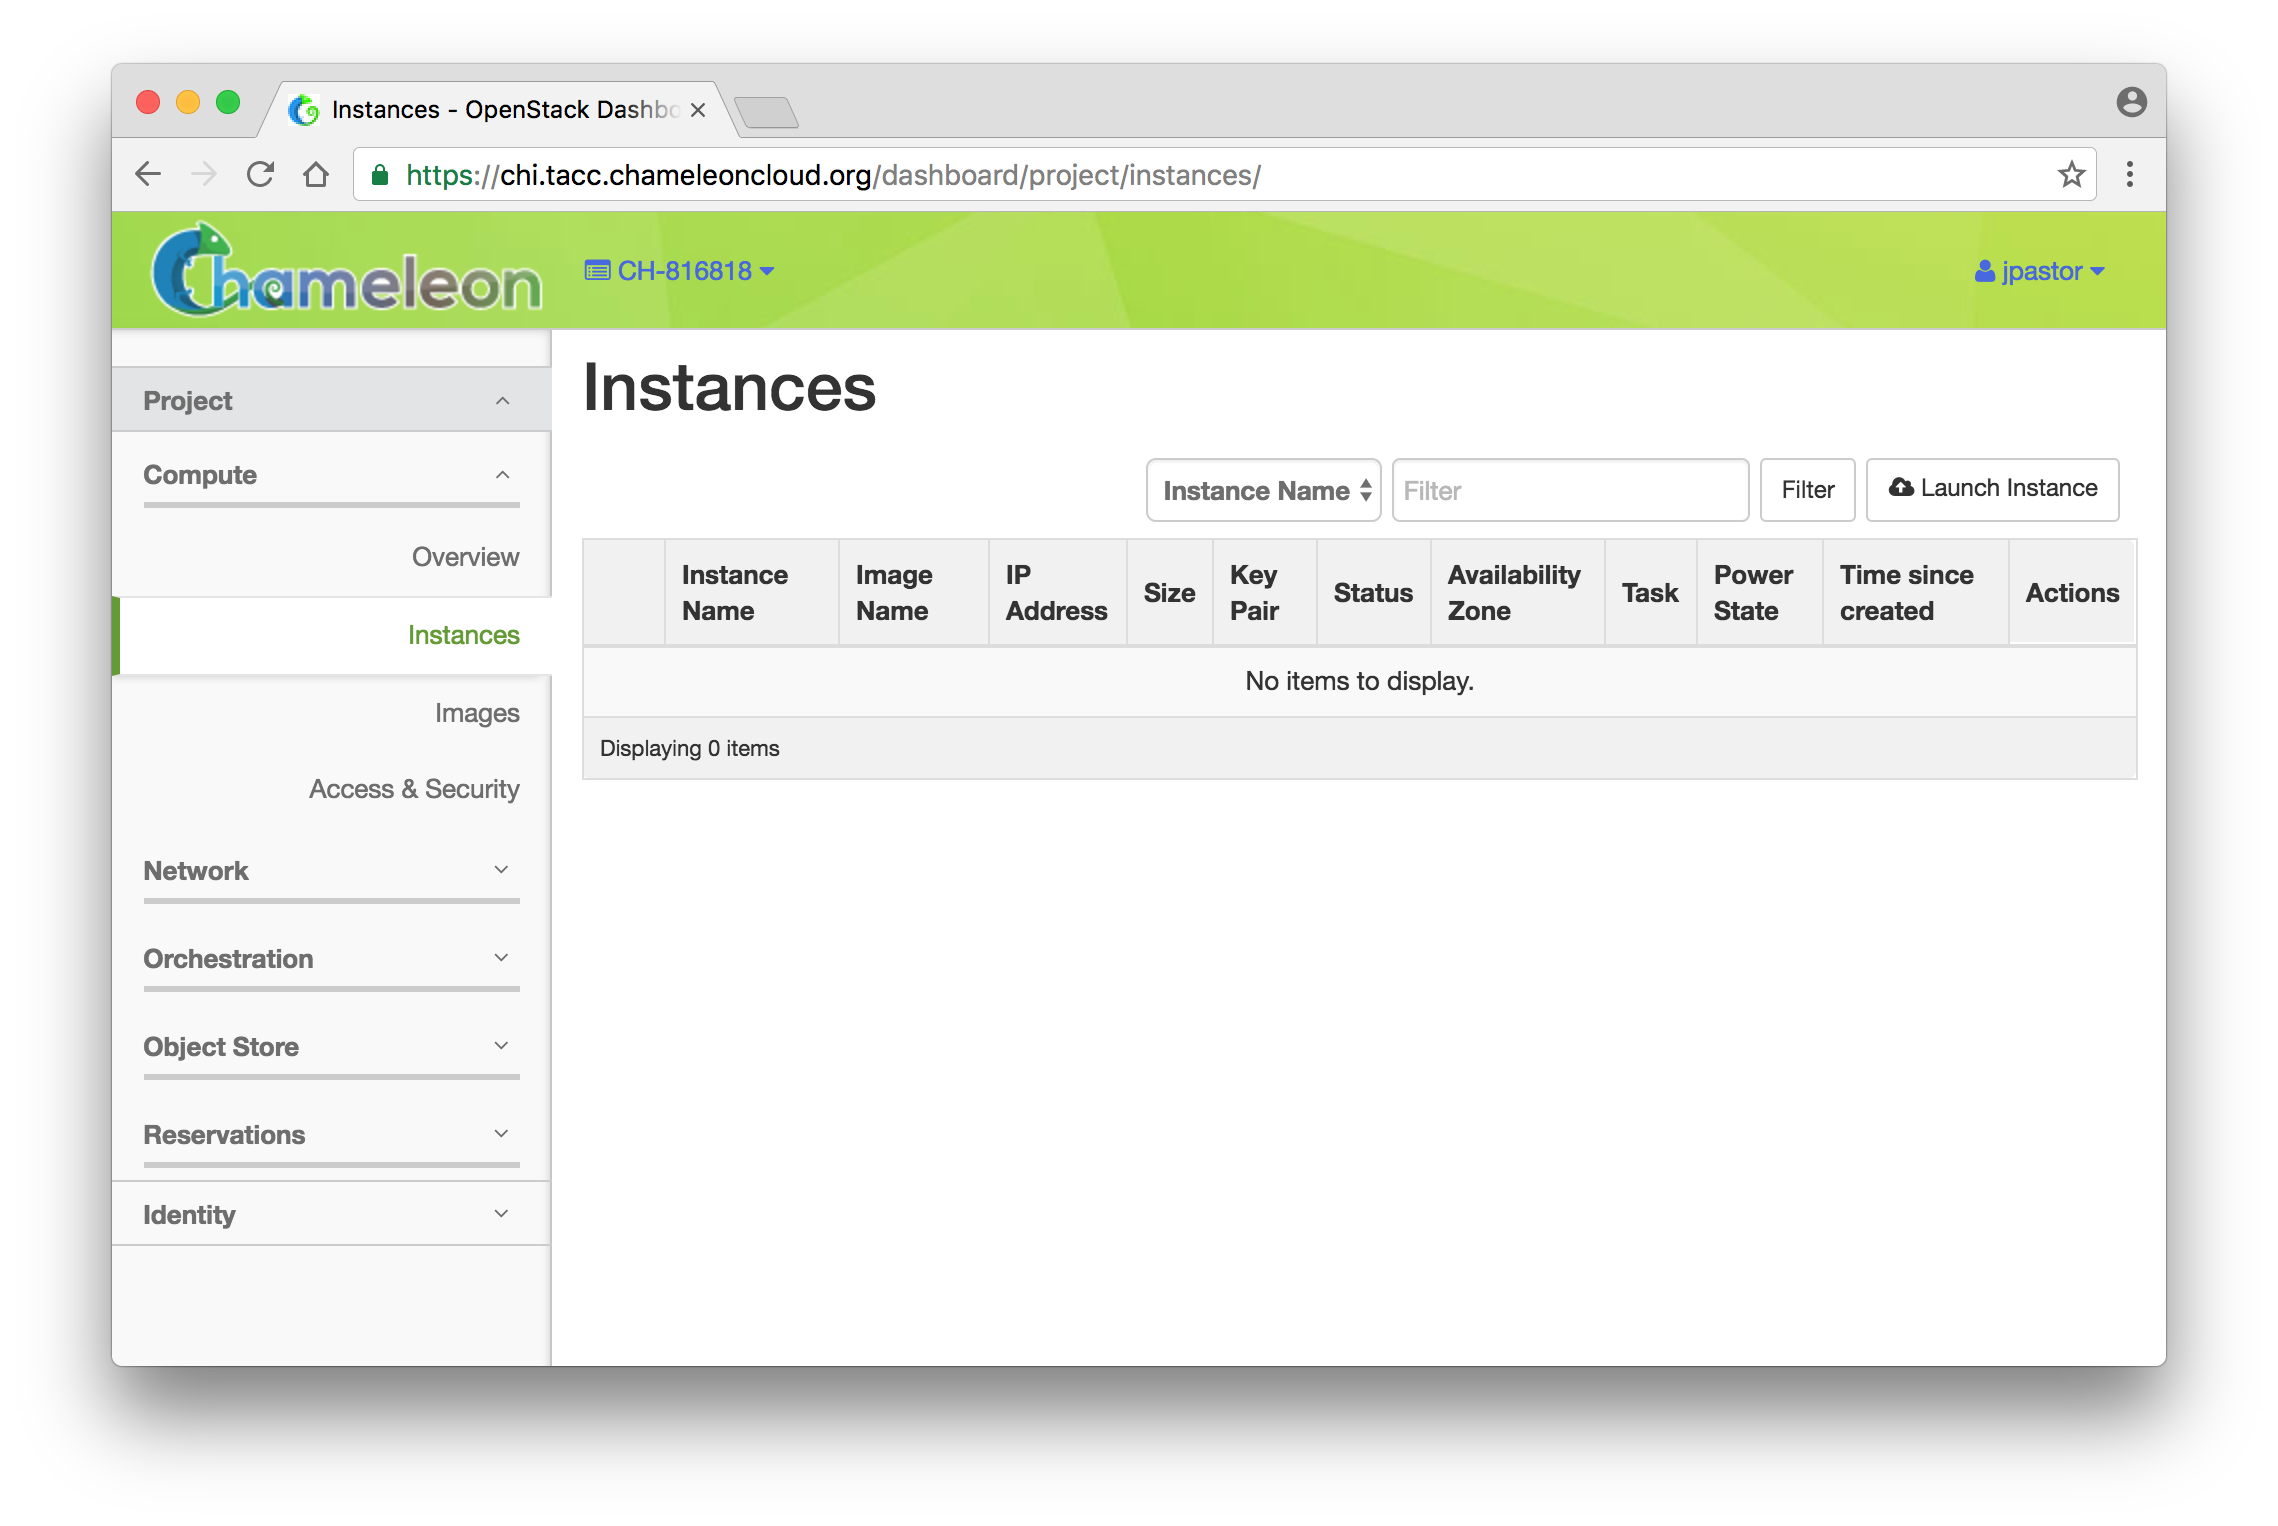
\includegraphics[width=\columnwidth]{images/chameleon/Screen-Shot-2016-10-26-at-14-39-56.png}

Click on the ``Launch Instance'' button in the top right corner. Select
a reservation in the Reservation box, pick an instance name (in this
example my-first-instance) and in~the Image Name list select our default
environment named CC-CentOS7. If you have multiple key pairs registered,
you need to select one in the ``Access \& Security''~tab. Finally, click
on the blue ``Launch'' button.

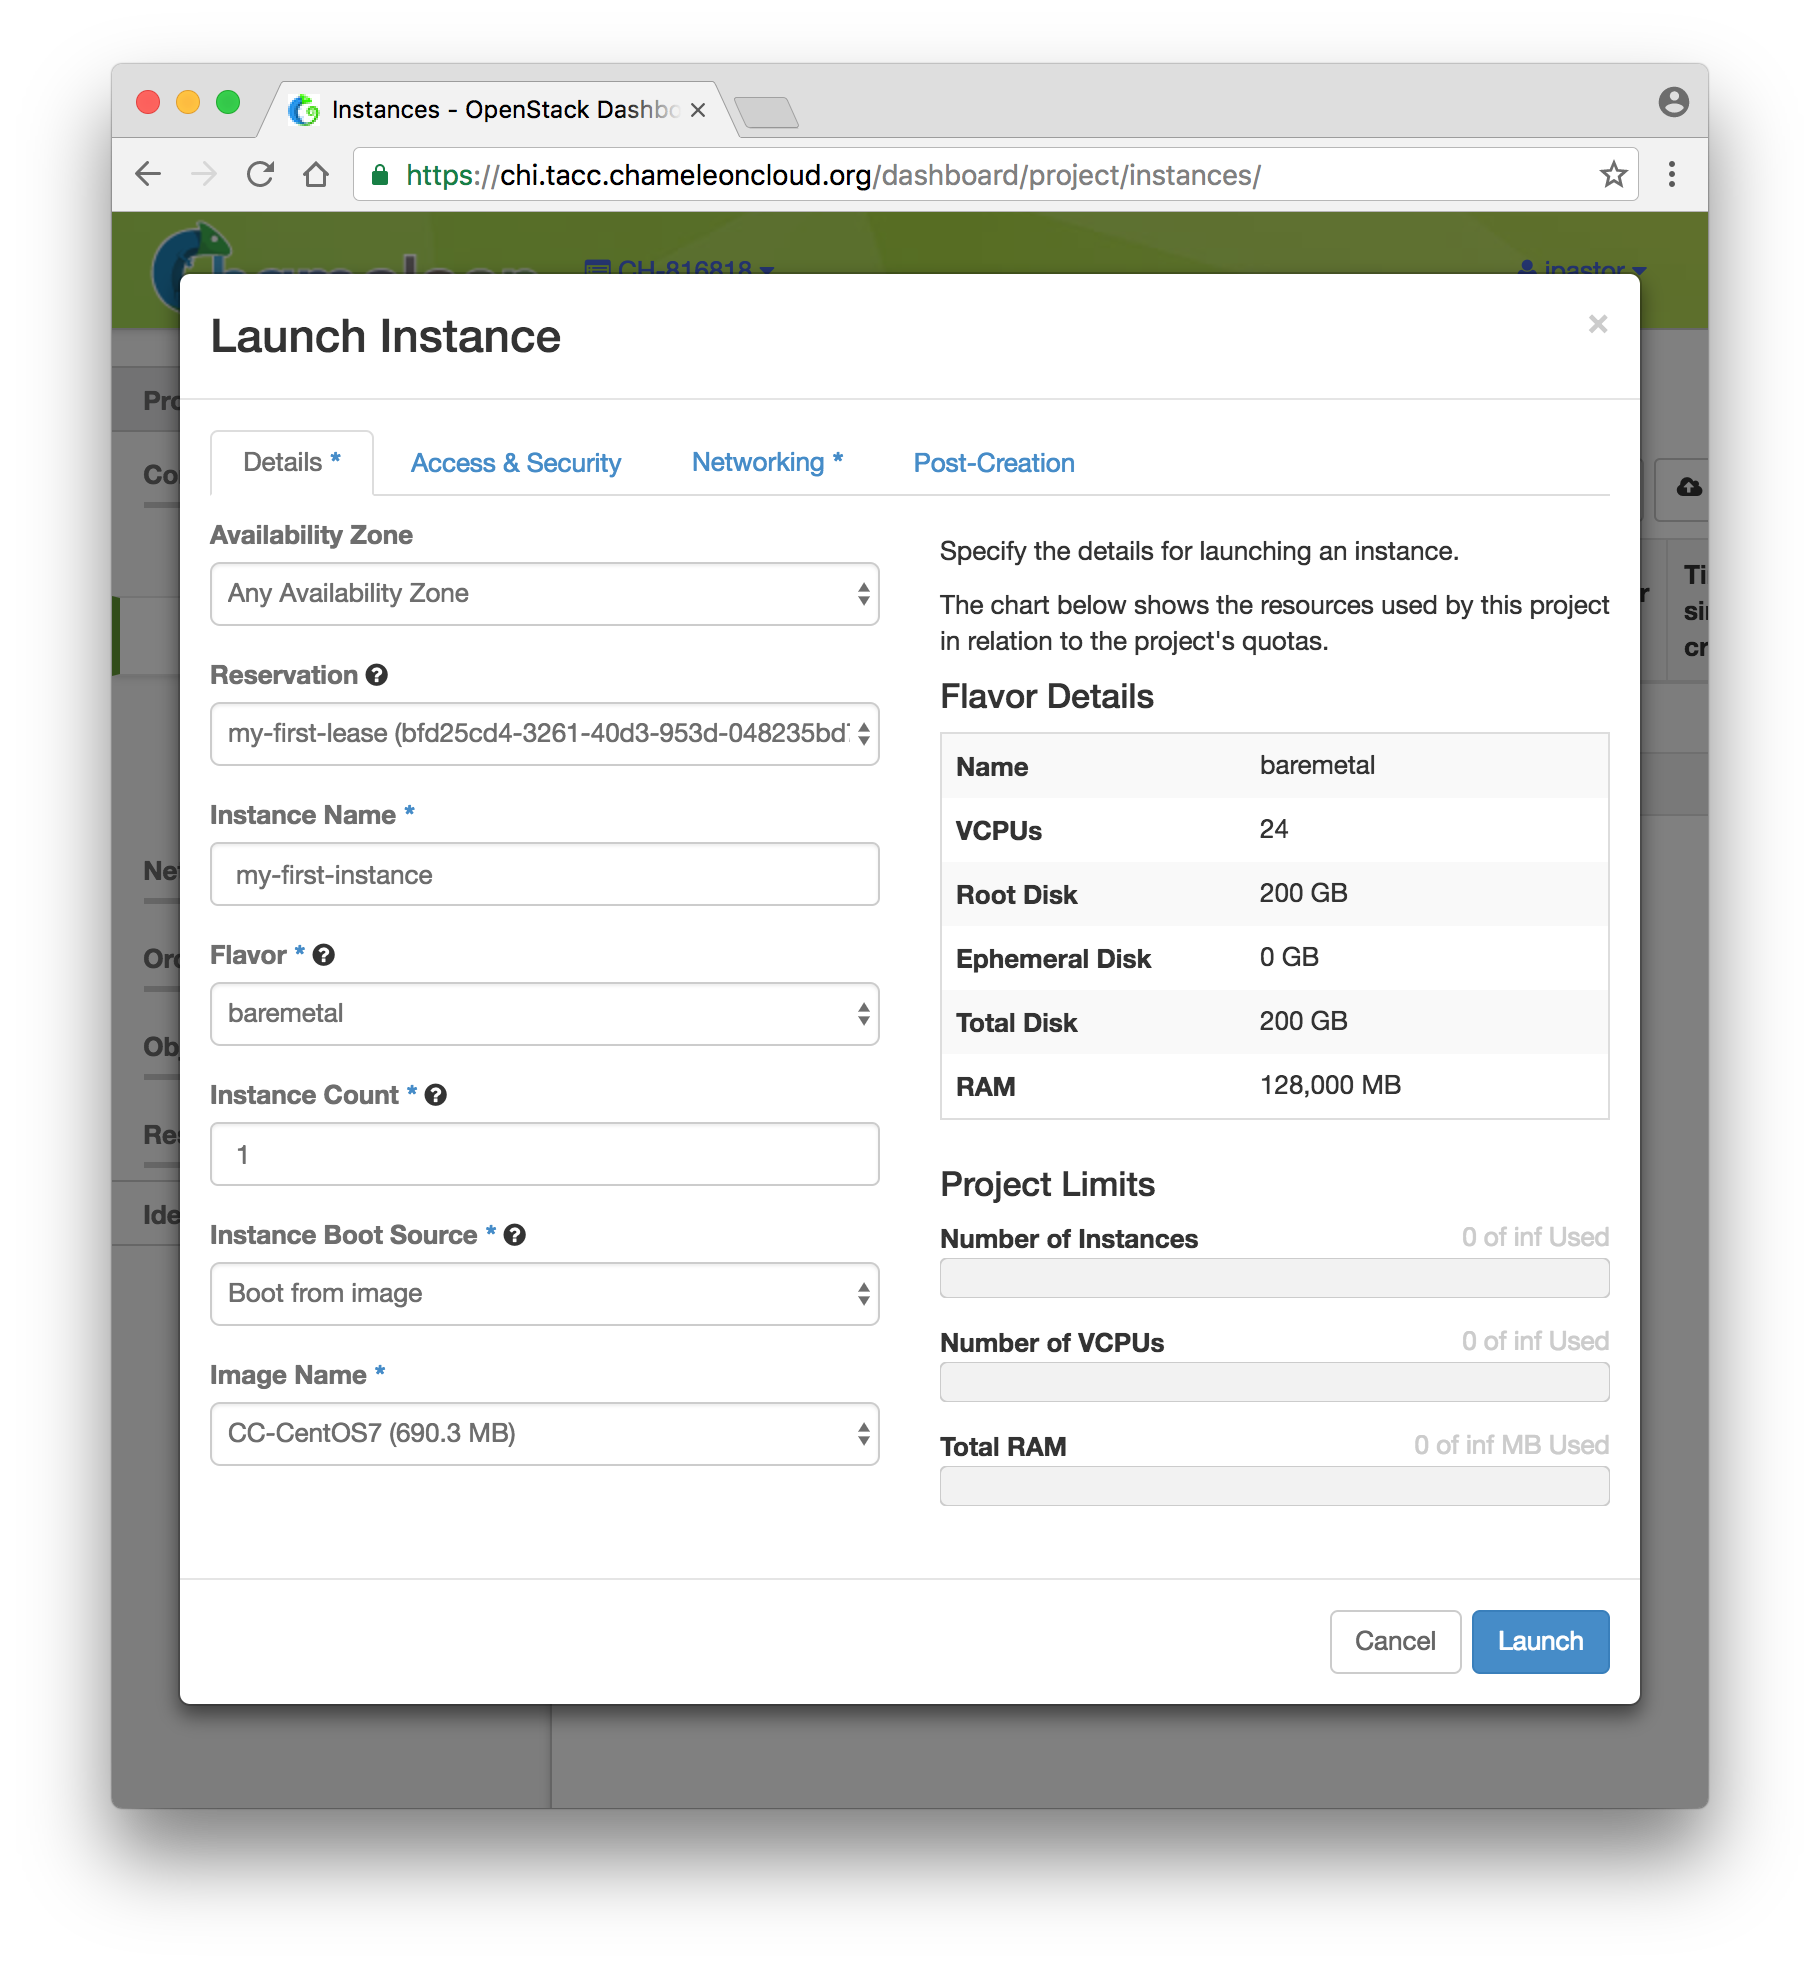
\includegraphics[width=\columnwidth]{images/chameleon/Screen-Shot-2016-10-26-at-14-41-08.png}

The instance will show up in the instance list, at first in Build
status. It takes a few minutes to deploy the instance on bare-metal
hardware and reboot the machine.

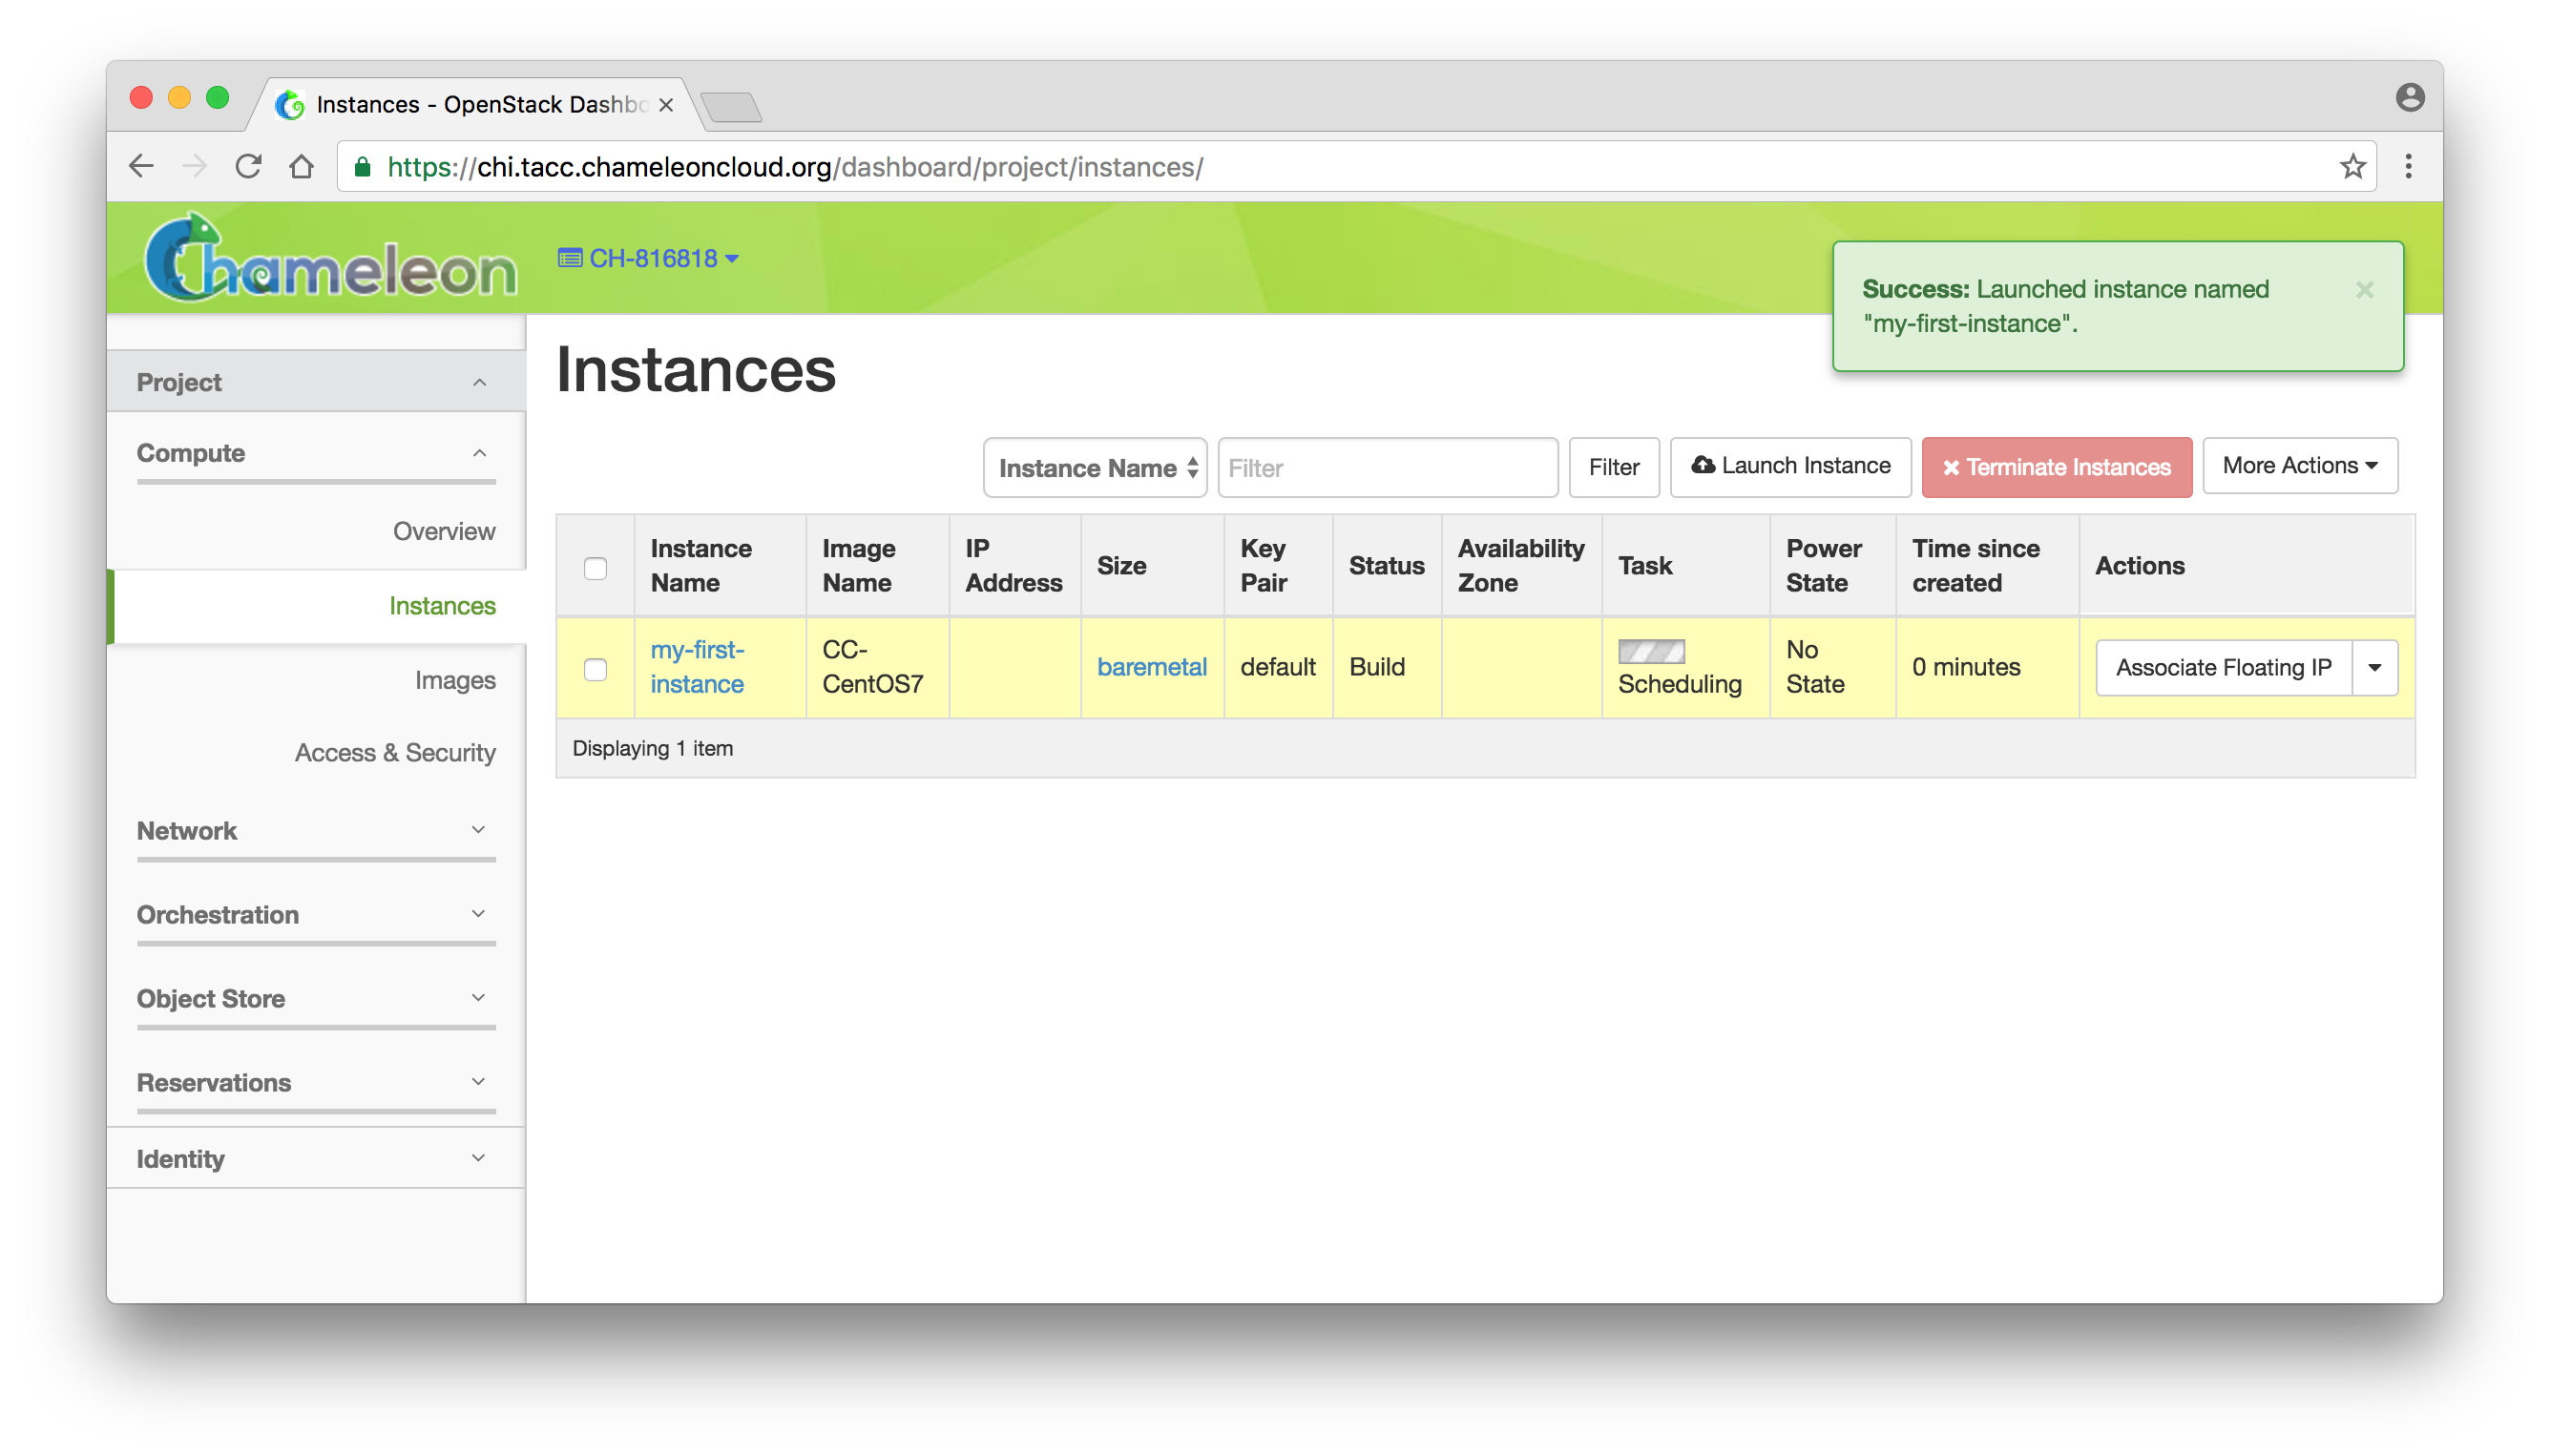
\includegraphics[width=\columnwidth]{images/chameleon/Screen-Shot-2016-10-26-at-15-53-31.png}

After a few minutes the instance should become in Active status and the
Power State should be Running.

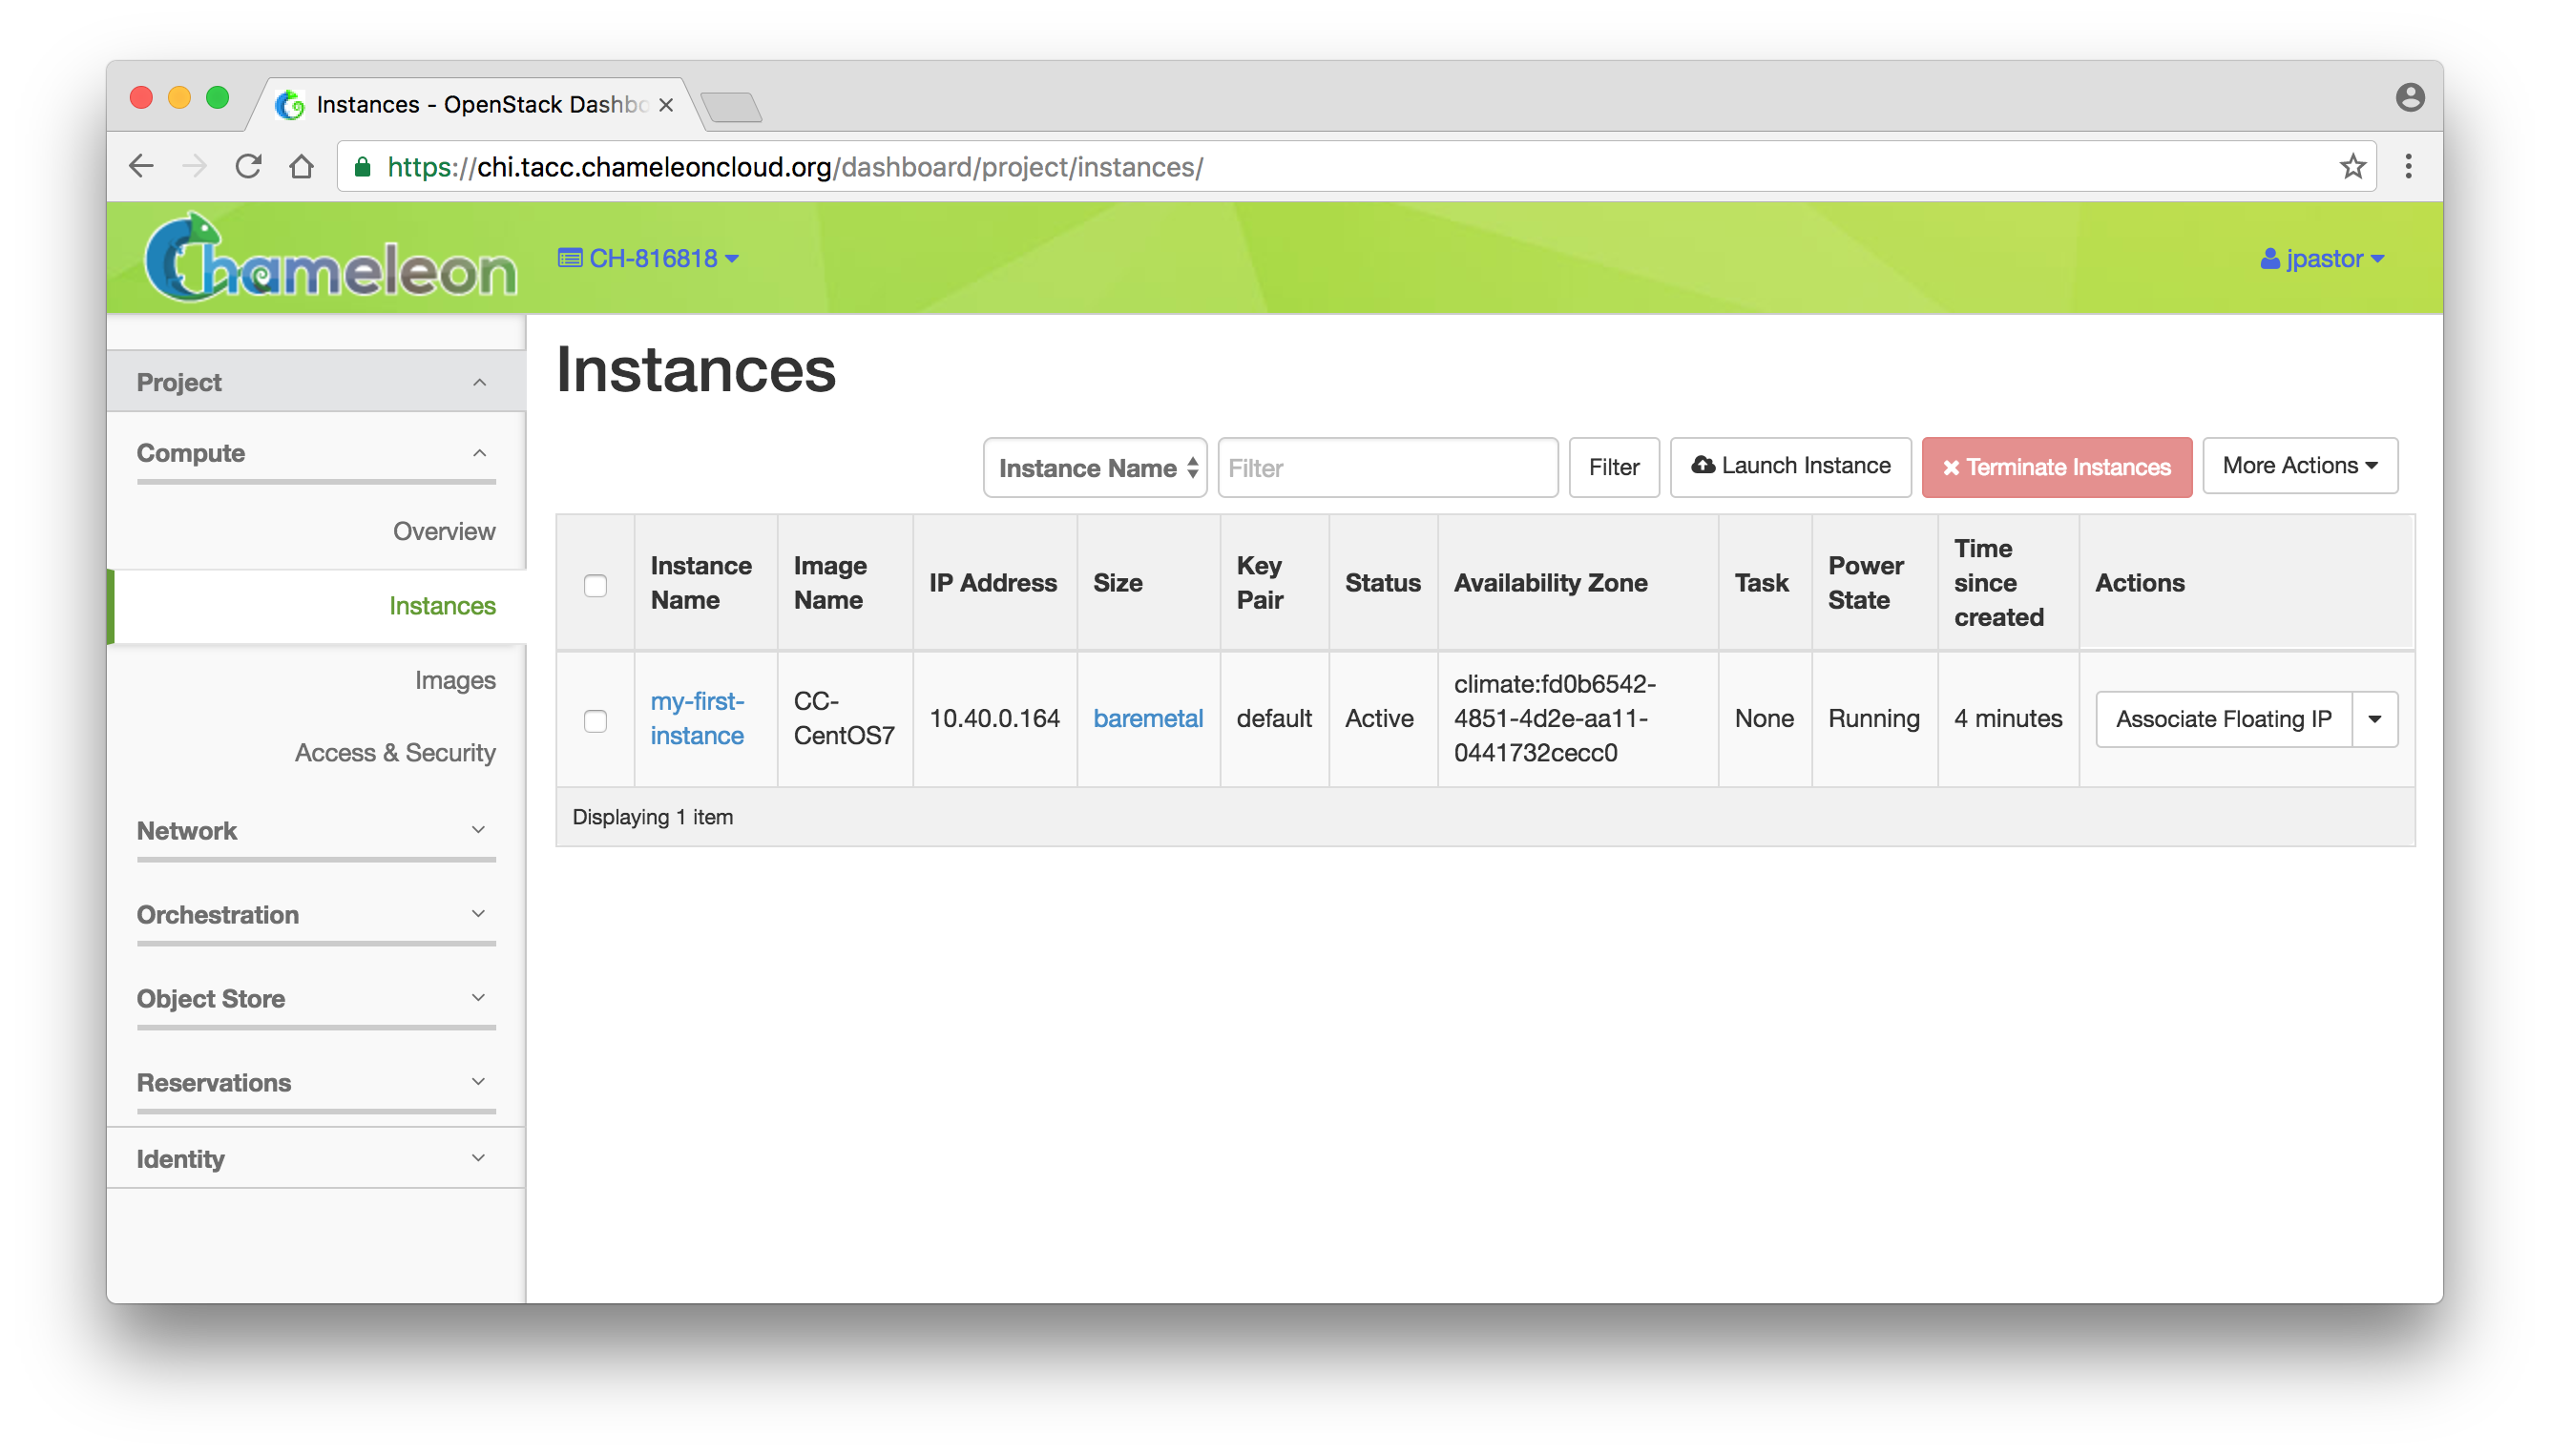
\includegraphics[width=\columnwidth]{images/chameleon/Screen-Shot-2016-10-26-at-16-22-38.png}

At this point the instance might still be booting: it might take a
minute or two to actually be accessible on the network and accept SSH
connections.~In the meantime, you can attach a floating IP to the
instance. Click on the~``Associate Floating IP'' button.~You should get
a screen like the one below:

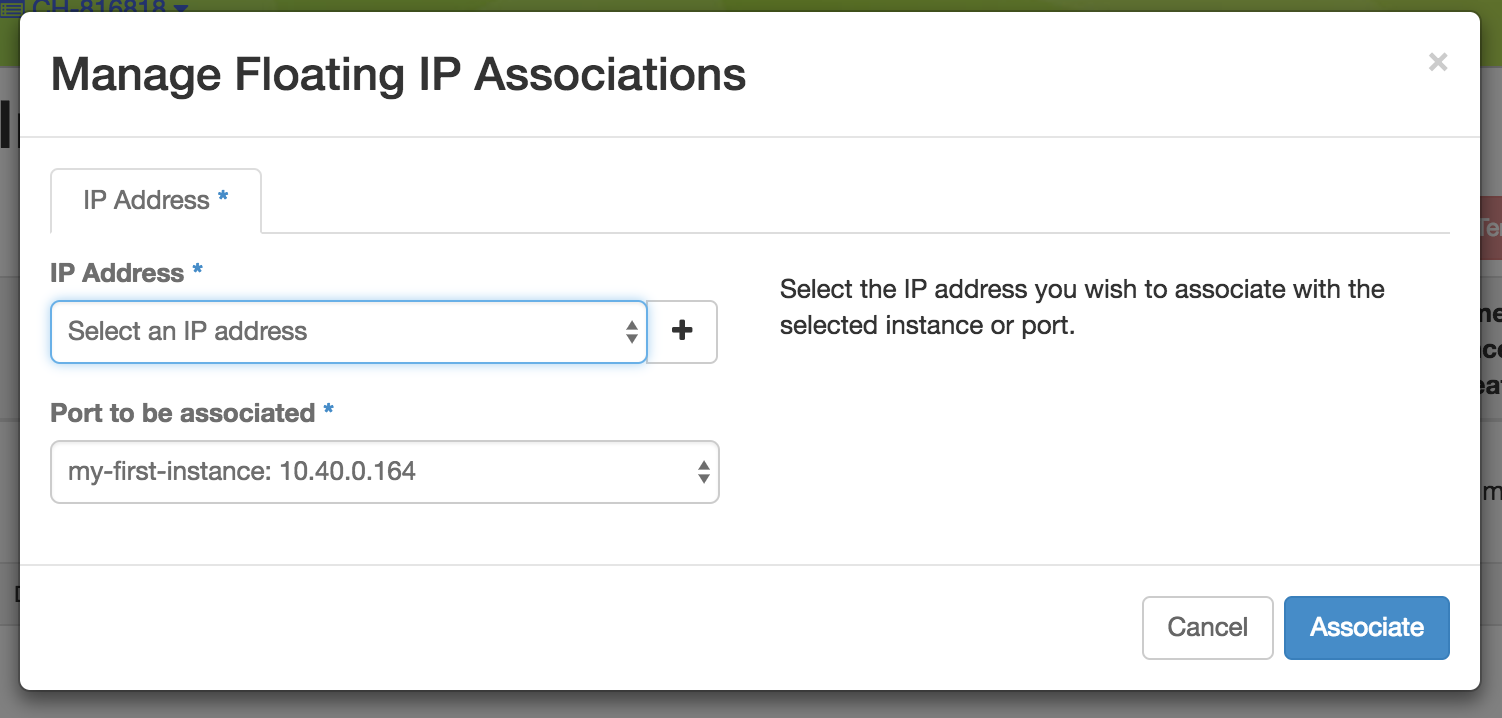
\includegraphics[width=\columnwidth]{images/chameleon/Screen-Shot-2016-10-26-at-16-25-04.png}

If there are no unused floating IP already allocated to your project,
click on the + button. In the window that opens, select the ext-net pool
if not already selected by default and click on the blue Allocate IP
button.

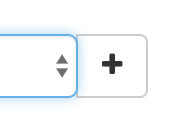
\includegraphics[width=\columnwidth]{images/chameleon/Screen-Shot-2016-10-26-at-16-33-45-W05kOLQ.png}

You will be returned to the previous window. The correct value for
``Port to be associated'' should already be selected, so you only have
to click on ``Associate''.

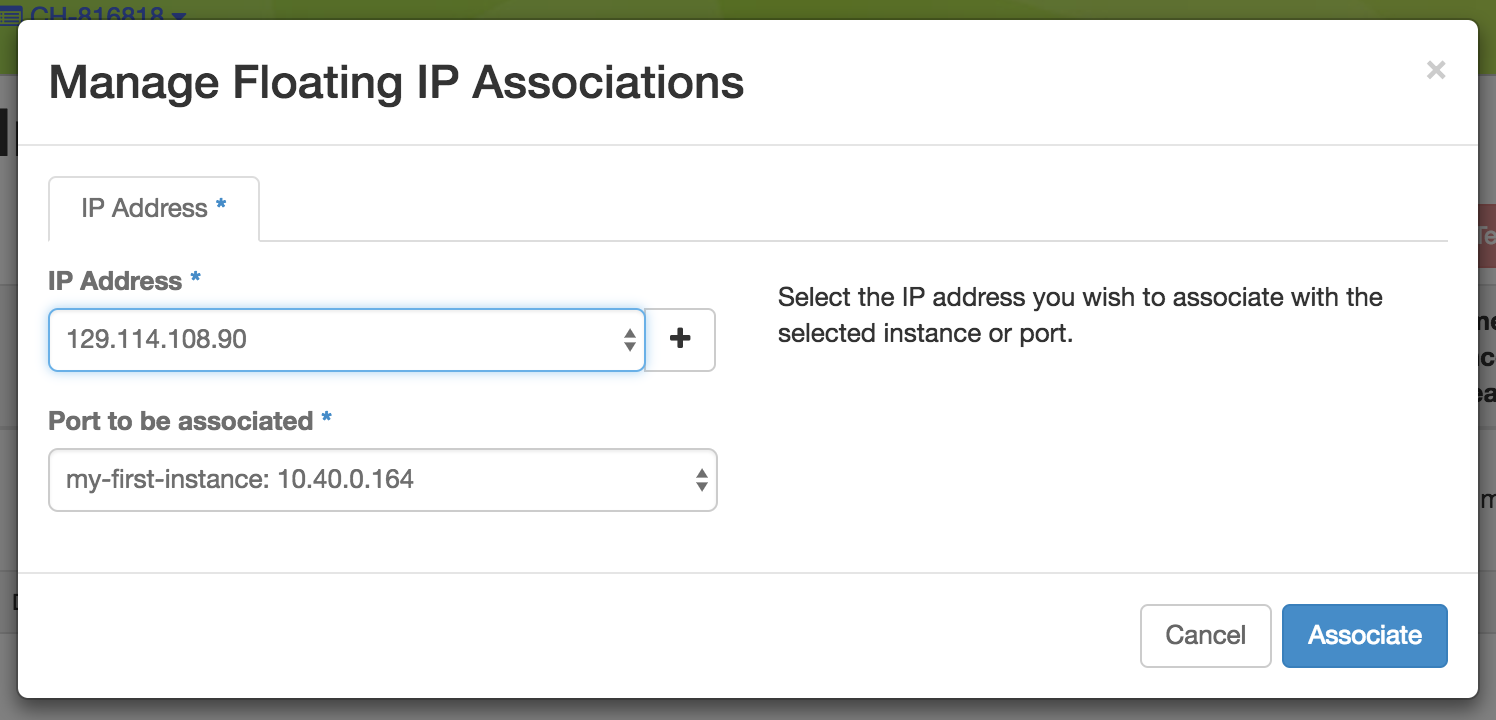
\includegraphics[width=\columnwidth]{images/chameleon/Screen-Shot-2016-10-26-at-16-25-10.png}

This should send you back to the instance list, where you can see the
floating IP attached to the instance (you may need to refresh your
browser to see the floating IP).

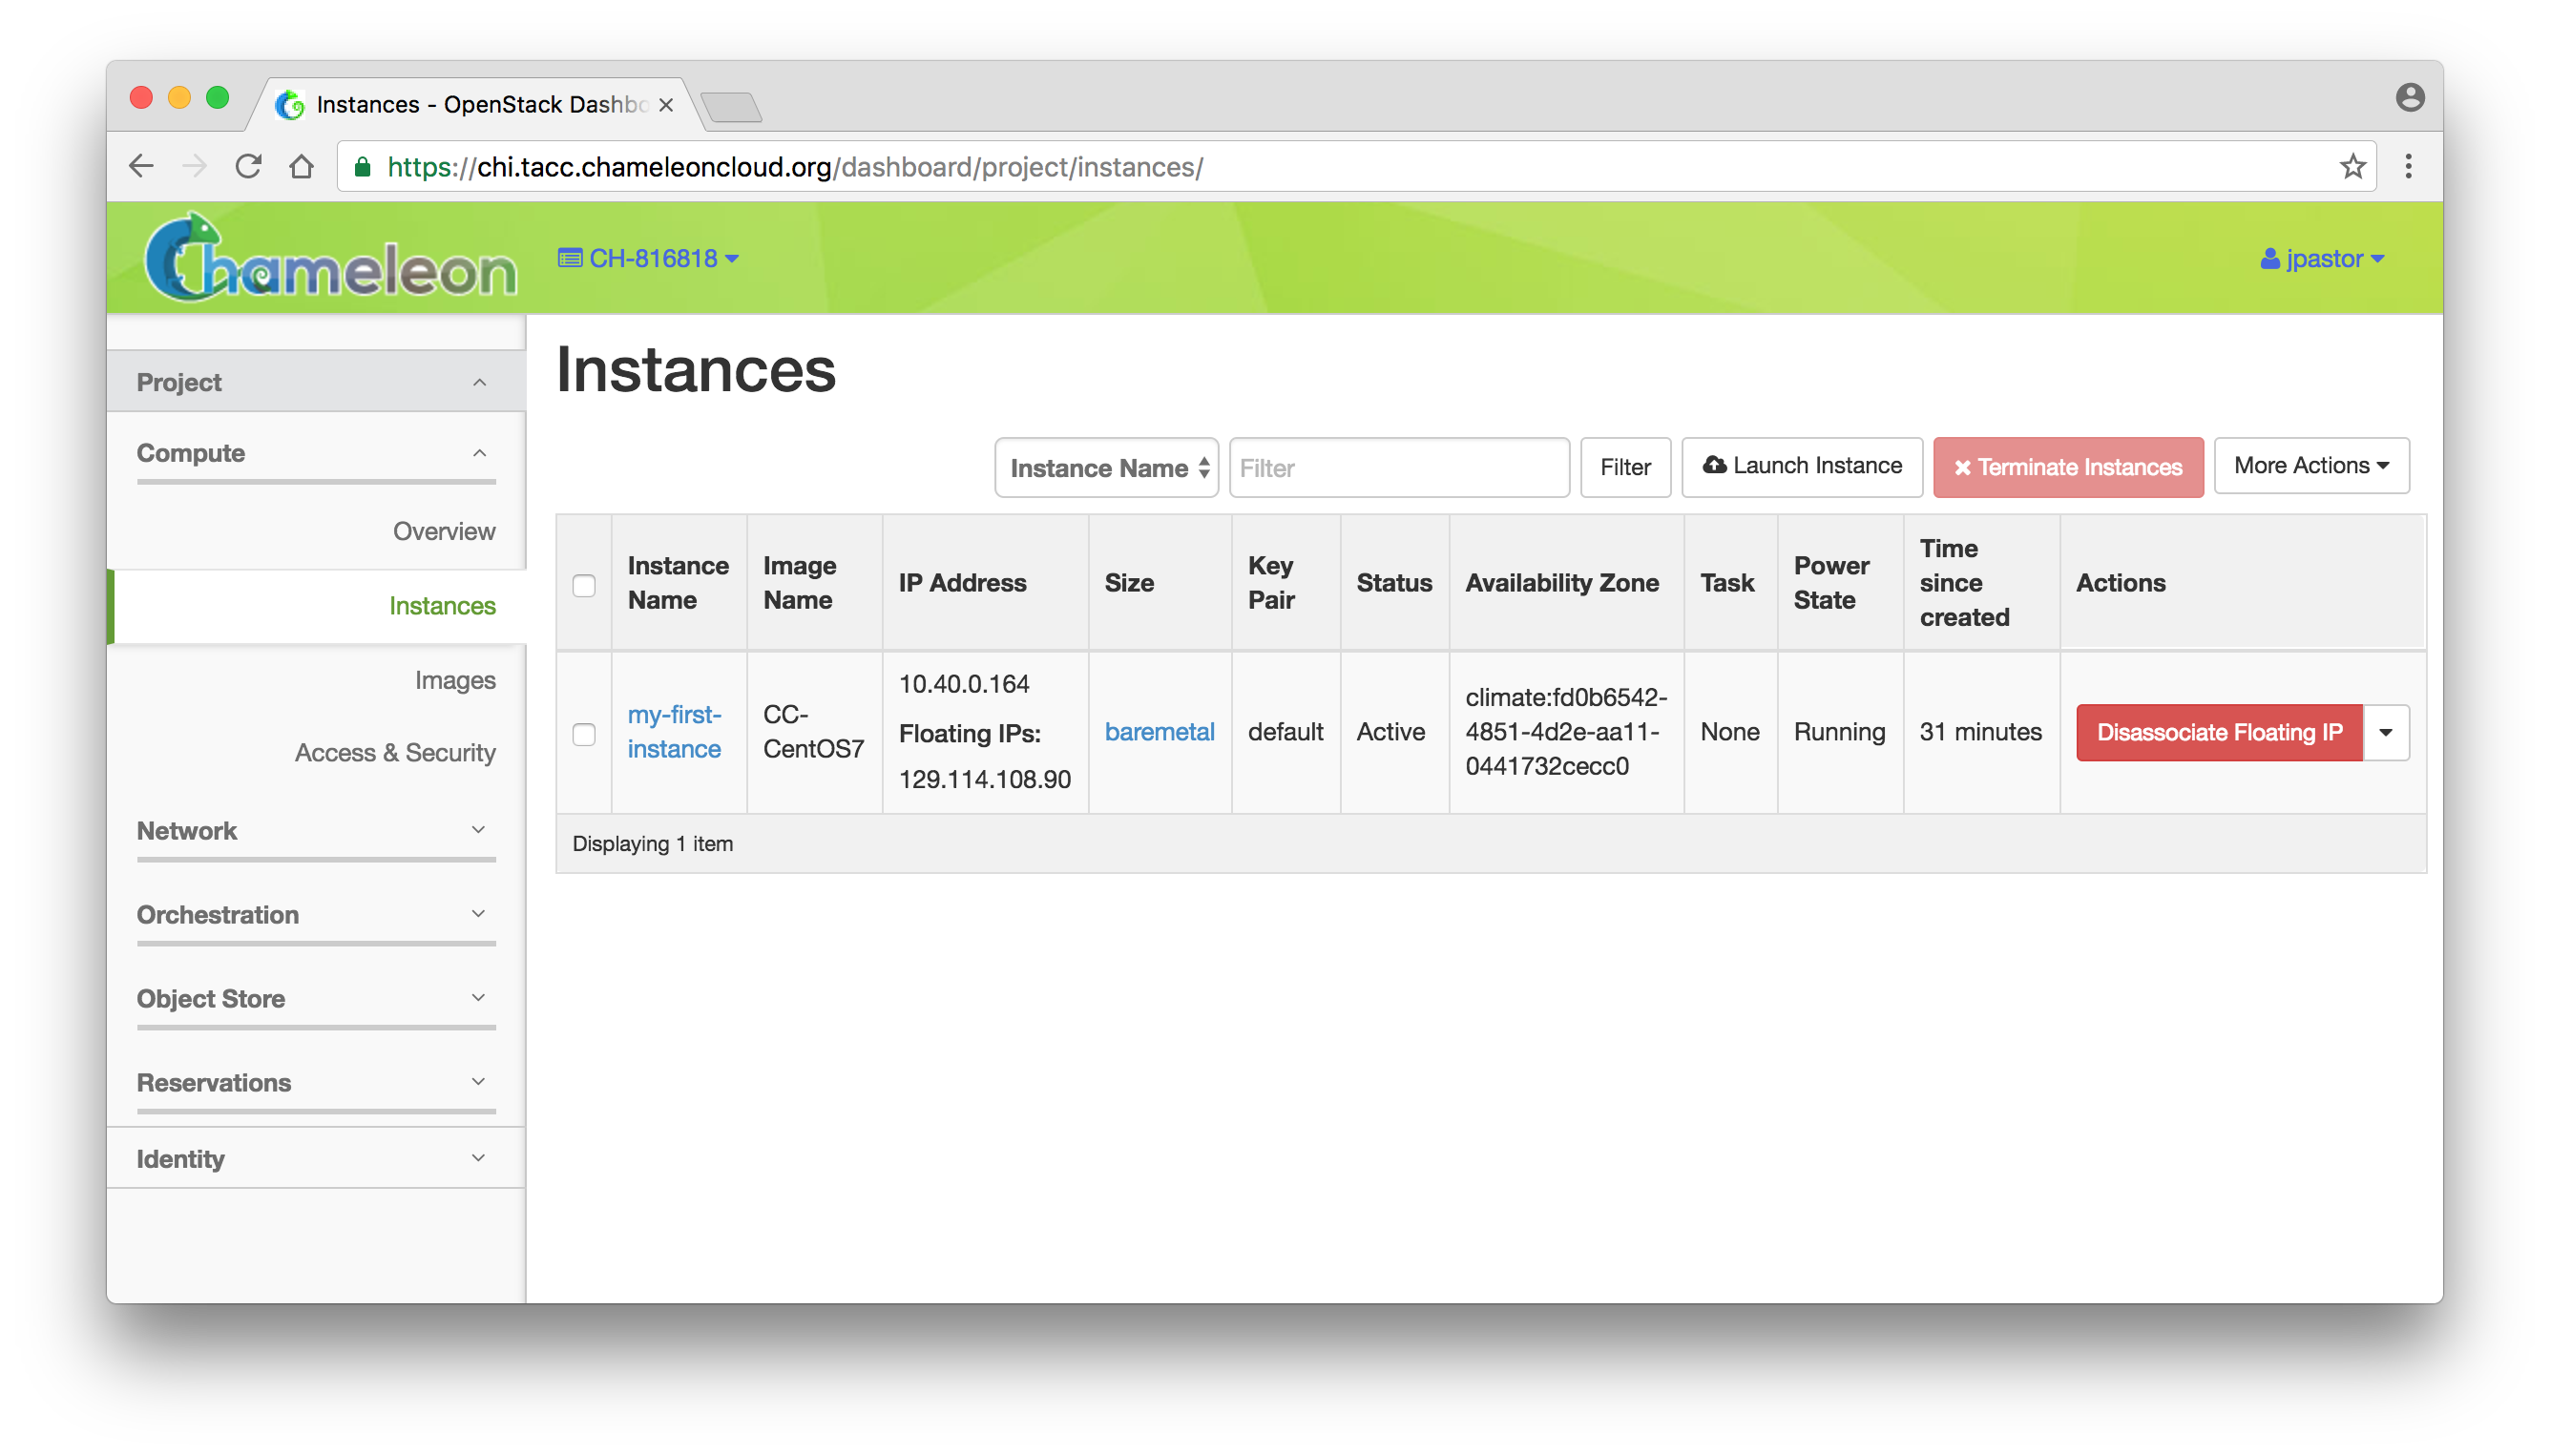
\includegraphics[width=\columnwidth]{images/chameleon/Screen-Shot-2016-10-26-at-16-26-54.png}

\section{Interact with resources}\label{interact-with-resources}

Now you should be able to connect to the instance via SSH using the cc
account. In a terminal, type ssh
cc@\textless{}floating\_ip\textgreater{}, in our example this would
be~\texttt{ssh\ cc@130.202.88.241}

SSH will probably tell you:

\begin{verbatim}
The authenticity of host \textquotesingle{}130.202.88.241
(130.202.88.241) can't be established. RSA key fingerprint 
is 5b:ca:f0:63:6f:22:c6:96:9f:c0:4a:d8:5e:dd:fd:eb. 
Are you sure you want to continue connecting (yes/no)?

\end{verbatim}

Type yes and press Enter. You should arrive to a prompt like this one:

\texttt{{[}cc@my-first-instance\ \textasciitilde{}{]}\$}

If you notice SSH errors such as connection refused, password requests,
or failures to accept your key, it is likely that the physical node is
still going through the boot process. In that case, please wait before
retrying. Also make sure that you use the~\textbf{cc}~account. If after
10 minutes you still cannot connect to the machine,
please~\href{https://www.chameleoncloud.org/user/help/}{open a ticket
with our help desk}.

You can now check whether the resource matches its known description in
the resource registry. For this, simply
run:~\texttt{sudo\ cc-checks\ -v}

{\centering 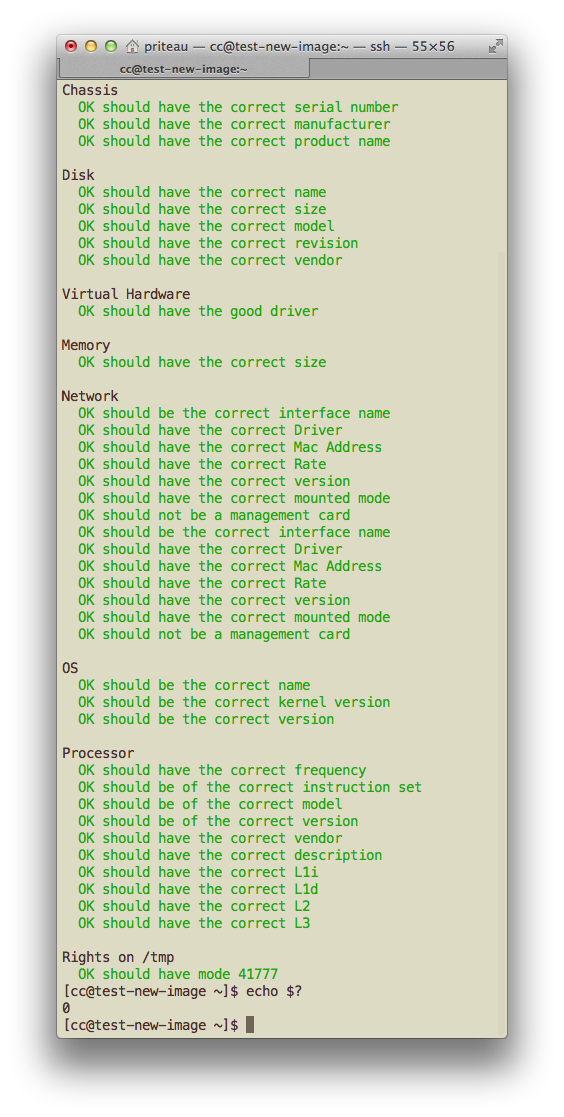
\includegraphics[width=0.5\columnwidth]{images/chameleon/cc-checks.png}}

The cc-checks program prints the result of each check in green if it is
successful and~red if it failed.

You can now run your experiment directly on the machine via SSH. You can
run commands with root privileges by prefixing them with~\texttt{sudo}.
To completely~switch~user and become root, use
the~\texttt{sudo\ su\ -\ root}~command.

\subsection{\texorpdfstring{{Snapshot an
instance}}{Snapshot an instance}}\label{snapshot-an-instance}

All instances in Chameleon, whether KVM or bare-metal, are running off
disk images. The content of these disk images can be snapshotted at any
point in time, which allows you to save your work and launch new
instances from updated images later.

While OpenStack KVM has built-in support for snapshotting in the Horizon
web interface and via the command line, bare-metal instances require a
more complex process. To make this process easier,{ we developed the
\href{https://github.com/ChameleonCloud/ChameleonSnapshotting}{cc-snapshot}
tool, which implements snapshotting a bare-metal instance from command
line and uploads it to Glance, so that it can be immediately used to
boot a new bare-metal instance. The snapshot images created with this
tool are whole disk images.}

{For ease of use, \emph{cc-snapshot} has been installed in all the
appliances supported by the Chameleon project. If you would like to use
it in a different setting, it can be downloaded and installed from the
\href{https://github.com/ChameleonCloud/ChameleonSnapshotting}{github
repository}.}

{Once cc-snapshot is installed, to make a snapshot of a bare-metal
instance, run the following command from inside the instance:}

{\texttt{sudo\ cc-snapshot\ \textless{}snapshot\_name\textgreater{}}}

{You can verify that it has been uploaded to Glance by running the
following command:}

{\texttt{glance\ image-list}}

{If you prefer to use a series of standard Unix commands, or are
generally interested in more detail about image management, please refer
to our
\href{https://www.chameleoncloud.org/docs/user-guides/ironic/\#snapshotting_an_instance}{image
management guide}.}

\section{Use FPGAs}\label{use-fpgas}

Consult the
\href{https://www.chameleoncloud.org/docs/bare-metal-user-guide/fpga/}{dedicated
page}~if you would like to use the FPGAs available on Chameleon.

\section{Next Step}\label{next-step}

Now that you have created some resources, it is time to interact with
them! You will find instructions to the next step by visiting the
following link:

\begin{itemize}
\tightlist
\item
  \href{https://www.chameleoncloud.org/monitor-and-collect/}{Monitor
  resources and collect results}
\end{itemize}


\FILENAME

\chapter{HEAT}\label{complex-appliances}

\section{What are complex~appliances?}\label{what-are-complexappliances}

Deploying an MPI cluster, an OpenStack installation, or any other type
of cluster in which nodes can take on multiple roles can be complex: you
have to provision potentially hundreds of nodes, configure them to take
on various roles, and make them share information that is generated or
assigned only at deployment time, such as hostnames, IP addresses, or
security keys. When you want to run a different experiment later you
have to redo all this work. When you want to reproduce the experiment,
or allow somebody else to reproduce it, you have to take very precise
notes and pay great attention to their execution.

To help solve this problem and facilitate reproducibility and sharing,
the Chameleon team configured a tool that allows you to deploy complex
clusters with ``one click''. This tool requires not just a simple image
(i.e., appliance) but also a document, called a template, that contains
the information needed to orchestrate the deployment and configuration
of such clusters. We call this image + template combination
complex~appliance because it consists of more than just the image (i.e.,
appliance).

\section{How are complex appliances
supported?}\label{how-are-complex-appliances-supported}

In a nutshell, complex appliances allow you to specify not only what
image you want to deploy but also on how many nodes you want to deploy
that image, what roles the deployed instances should boot into (such as
e.g., head node and worker node in a cluster), what information from a
specific instance should be passed to another instance in that complex
appliance, and what scripts should be executed on boot so that this
information is properly used for configuring the ``one click'' cluster.
For example, a Network File System (NFS) appliance that we will use as
an example in this guide, might specify deployment on three nodes, out
of which one will be configured as head node and others as worker nodes,
the information passed between the images will be hostname of the head
node, and the scripts executed on the worker nodes on boot will put that
hostname in the fstab file. As you can tell from this description,
images used for complex appliances are typically configured such that
they can be booted into any role required on the one-click cluster we
are booting; in this case the image will have both the software for NFS
server node and client~node.

Since complex appliances in Chameleon are currently implemented using
the \href{https://wiki.openstack.org/wiki/Heat}{OpenStack Heat}
orchestration service, we will be using OpenStack terminology and
features to work with them. The templates described above are YAML files
using the
\href{http://docs.openstack.org/developer/heat/template_guide/hot_spec.html}{Heat
Orchestration Template (HOT) format} (Heat also supports the AWS
CloudFormation template format, but this is not covered here). A
deployed complex appliance is referred to as a ``stack'' -- just as a
deployed single appliance is typically referred to as an ``instance''.
This guide will tell you all you need to know in order to use and
configure complex appliances on Chameleon; if you would like to know
more about Heat, please refer to its
\href{http://docs.openstack.org/developer/heat/}{official
documentation}.

\section{Where can I find Chameleon complex
appliances?}\label{where-can-i-find-chameleon-complex-appliances}

Our \href{https://www.chameleoncloud.org/appliances/}{Appliance Catalog}
has several complex appliances for popular technologies that people want
to deploy such as OpenStack or MPI or even more advanced deployments
such as efficient SR-IOV enabled MPI in KVM virtual machines. We also
provide common building blocks for cluster architectures, such as an NFS
share. Complex appliances are identified by a badge in their top-right
corner representing a group of machines, as shown in the screenshot:

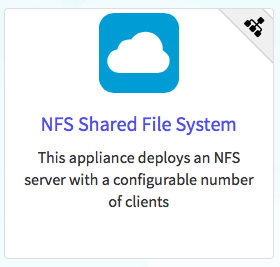
\includegraphics[width=0.5\columnwidth]{images/chameleon/NFS.png}

\section{How do I deploy a complex
appliance?}\label{how-do-i-deploy-a-complex-appliance}

We will explain how to launch a complex appliance based on our
\href{https://www.chameleoncloud.org/appliances/25/}{NFS share
appliance}. To launch a complex appliance, you only need to follow these
steps:

\begin{enumerate}
\item
  Create a lease: use the OpenStack web interface (choose between CHI@UC
  or CHI@TACC) to create a lease. To launch our NFS appliance, reserve
  at least three compute nodes (the strict minimum is two nodes but we
  will use three in this example and later ones).
\item
  Go to the \href{https://www.chameleoncloud.org/appliances/}{Appliance
  Catalog} and identify the appliance you want to launch. In our case
  you can go straight to the
  \href{https://www.chameleoncloud.org/appliances/25/}{NFS
  share~appliance}; click on it to open its details page. You will see a
  ``Launch'' button and a ``Get Template'' button. Follow the ``Get
  Template'' link and copy its url to the clipboard --~you will need it
  in the following steps.
\item
  Click on the ``Launch Complex Appliance at CHI@TACC'' or ``Launch
  Complex Appliance at CHI@UC'' button depending on where your
  reservation was created.
\end{enumerate}

This will take you to the Stacks page within the Orchestration menu.
This page will show the current list of stacks, with controls to manage
them and create new ones. Since we haven't launched any yet, this list
will be empty for now.

We will now create a new stack, which corresponds to the launch of a
template. Click on Launch Stack on the top right. A window will pop up
like below:

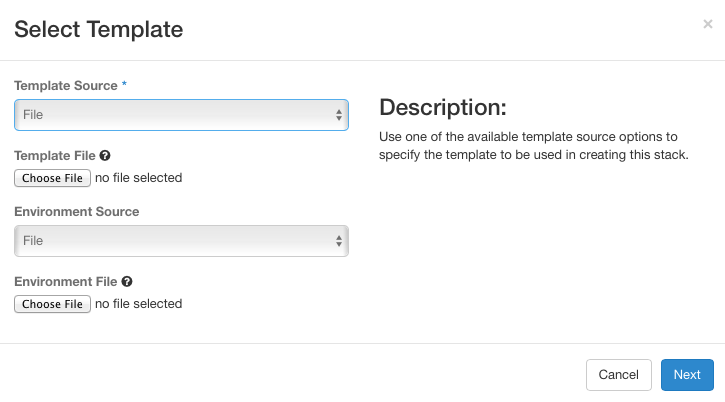
\includegraphics[width=\columnwidth]{images/chameleon/Launch-Stack.png}

We will deploy the NFS appliance described earlier; it will consist of a
server node and two client nodes. Change the template source field to
URL, and paste the URL of the
\href{https://www.chameleoncloud.org/appliances/api/appliances/25/template}{NFS
share~template} (if you don't have it in your clipboard anymore you will
need to go back to the appliance and get it by clicking on ``Get
template'' again).

Don't change the environment source settings, and click ``Next''.

The next screen allows your to enter input values to your Heat template.
Choose a name for your stack (e.g. my-nfs-cluster). Ignore the
``Creation Timeout'' and ``Rollback On Failure'' settings. You also need
to enter your Chameleon password. Then, you need to select a value for
the three parameters of the template: for key\_name, choose your SSH key
pair (this key pair will authorize access on each deployed instances,
both server and client). For nfs\_client\_count, change the default
value of 1 to 2. For reservation\_id, choose your reservation created
earlier. Finally, click ``Launch''.

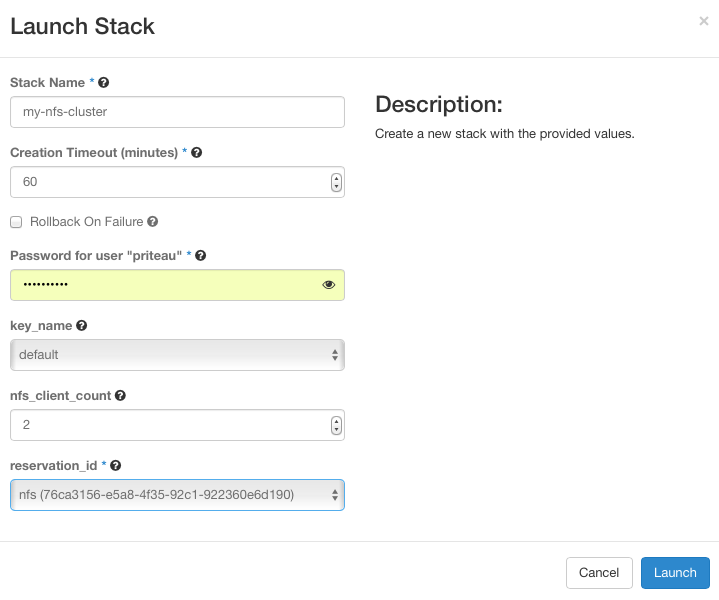
\includegraphics[width=\columnwidth]{images/chameleon/Launch-NFS-Stack.png}

Your stack should be in status ``Create In Progress'' for several
minutes while it first launches the NFS server instance, followed by the
NFS client instances.

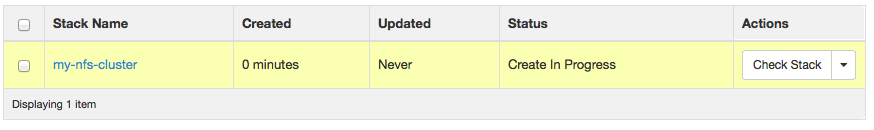
\includegraphics[width=\columnwidth]{images/chameleon/Create-In-Progress_zPgOjo4.png}

It will then move to the status ``Create Complete''.

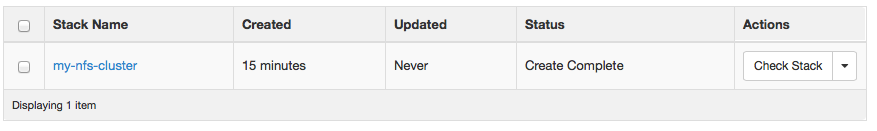
\includegraphics[width=\columnwidth]{images/chameleon/Create-Complete_XkoWhlj.png}

You can click on the stack name to get more details, including a
visualization of the deployed resources, as pictured below. The single
machine inside a circle represents the NFS server instance. The rack of
machine represents the group of NFS client instances (in this case, a
group composed of two instances). The server's floating IP (the public
IP assigned to a resource) is represented by an IP in a circle; an~IP in
a circle is also used to represent the association of the IP with~the
NFS server instance (not the greatest idea to use the same symbol for
both the IP and the association -- we agree but can't do much about it
at the moment). Blow off some steam by dragging the visualization across
the screen, it can be rather fun!

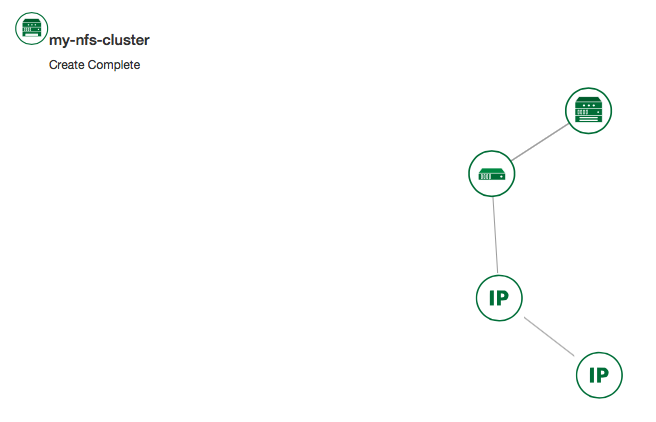
\includegraphics[width=\columnwidth]{images/chameleon/Stack-visualization.png}

You can now ssh to the server using the floating IP just as you do with
regular instances (use the cc account). The client does not have a
floating IP attached to it (as per the visualization above) but you can
connect to it via the server node with the client's private IP (connect
to the server with \texttt{ssh\ -A}~to enable the SSH agent forwarding
after loading your key to your SSH agent
with~\texttt{ssh-add\ \textless{}path-to-your-key\textgreater{}}).

You can find out the information about the IPs and other things if you
click the ``Overview'' tab and look in the ``Outputs'' section. Under
the ``Resources'' tab you will see the resources described above (the
server, clients, server's public/floating IP, and its the association)
and information about them. In the ``Events'' tab you will see
information about the history of the deployment so far. In Template you
will see the template that was used to deploy this stack.

\section{What is inside a Heat
template?}\label{what-is-inside-a-heat-template}

The NFS share appliance deploys:

\begin{itemize}
\item
  an NFS server instance, that exports the directory /exports/example to
  any instance running on Chameleon bare-metal,
\item
  one or several NFS client instances, which configure /etc/fstab to
  mount this NFS share to /mnt (and can subsequently read from and write
  to it).
\end{itemize}

This template is reproduced further below, and includes inline comments
starting with the \# character. There are three main sections:

\begin{itemize}
\item
  resources,
\item
  parameters,
\item
  outputs.
\end{itemize}

The resources section is the most important part of the template: it
defines which OpenStack resources to create and configure. Inside this
section you can see four resources defined:

\begin{itemize}
\item
  nfs\_server\_floating\_ip
\item
  nfs\_server~
\item
  nfs\_server\_ip\_association
\item
  nfs\_clients
\end{itemize}

The first resource, nfs\_server\_floating\_ip, creates a floating IP on
the ext-net public network. It is not attached to any instance yet.

The second resource, nfs\_server, creates the NFS server instance (an
instance is defined with the type \texttt{OS::Nova::Server} in Heat). It
is a bare-metal instance (\texttt{flavor:\ baremetal}) using the
CC-CentOS7 image and connected to the private network named sharednet1.
We set the keypair to use the value of the parameter defined earlier,
using the \texttt{get\_param} function. Similarly, the reservation to
use is passed to the scheduler. Finally, a user-data script is given to
the instance, which configures it as an NFS server exporting
/exports/example to Chameleon instances.

The nfs\_server\_ip\_association resource associates the floating IP
created earlier with the NFS server instance.

Finally, the nfs\_clients resource defines a resource group containing
instance configured to be NFS clients and mount the directory exported
by the NFS server defined earlier. The IP of the NFS server is gathered
using the \texttt{get\_attr} function, and placed into user-data using
the \texttt{str\_replace} function.

Parameters all have the same data structure: each one has a name
(\texttt{key\_name} or \texttt{reservation\_id} in this case), a data
type (number or string), a comment field called description, optionally
a default value, and a list of constraints (in this case only one per
parameter). Constraints tell Heat to match a parameter to a specific
type of OpenStack resource. Complex appliances on Chameleon require
users to customize at least the key pair name and reservation ID, and
will generally provide additional parameters to customize other
properties of the cluster, such as its size, as in this example.

Outputs are declared similarly to parameters: they each have a name, an
optional~description, and a value. They allow to return information from
the~stack to the user.

\begin{footnotesize}
\begin{verbatim}
# This describes what is deployed by this template.
description: NFS server and clients deployed with Heat on Chameleon

# This defines the minimum Heat version required by this template.
heat_template_version: 2015-10-15

# The resources section defines what OpenStack resources are to be deployed and
# how they should be configured.
resources:
  nfs_server_floating_ip:
    type: OS::Nova::FloatingIP
    properties:
      pool: ext-net

  nfs_server:
    type: OS::Nova::Server
    properties:
      flavor: baremetal
      image: CC-CentOS7
      key_name: { get_param: key_name }
      networks:
         - network: sharednet1
      scheduler_hints: { reservation: { get_param: reservation_id } }
      user_data: |
        #!/bin/bash
        yum install -y nfs-utils
        mkdir -p /exports/example
        chown -R cc:cc /exports
        echo '/exports/example 10.140.80.0/22(rw,async) 10.40.0.0/23(rw,async)' >> /etc/exports
        systemctl enable rpcbind && systemctl start rpcbind
        systemctl enable nfs-server && systemctl start nfs-server

  nfs_server_ip_association:
    type: OS::Nova::FloatingIPAssociation
    properties:
      floating_ip: { get_resource: nfs_server_floating_ip }
      server_id: { get_resource: nfs_server }

  nfs_clients:
    type: OS::Heat::ResourceGroup
    properties:
      count: { get_param: nfs_client_count }
      resource_def:
        type: OS::Nova::Server
        properties:
          flavor: baremetal
          image: CC-CentOS7
          key_name: { get_param: key_name }
          networks:
             - network: sharednet1
          scheduler_hints: { reservation: { get_param: reservation_id } }
          user_data:
            str_replace:
              template: |
                #!/bin/bash
                yum install -y nfs-utils
                echo "$nfs_server_ip:/exports/example    /mnt/    nfs" > /etc/fstab
                mount -a
              params:
                $nfs_server_ip: { get_attr: [nfs_server, first_address] }

# The parameters section gathers configuration from the user.
parameters:
  nfs_client_count:
    type: number
    description: Number of NFS client instances
    default: 1
    constraints:
      - range: { min: 1 }
        description: There must be at least one client.
  key_name:
    type: string
    description: Name of a KeyPair to enable SSH access to the instance
    default: default
    constraints:
    - custom_constraint: nova.keypair
  reservation_id:
    type: string
    description: ID of the Blazar reservation to use for launching instances.
    constraints:
    - custom_constraint: blazar.reservation

outputs:
  server_ip:
    description: Public IP address of the NFS server
    value: { get_attr: [nfs_server_floating_ip, ip] }
  client_ips:
    description: Private IP addresses of the NFS clients
    value: { get_attr: [nfs_clients, first_address] }
\end{verbatim}
\end{footnotesize}

\section{Customizing an existing
template}\label{customizing-an-existing-template}

Customizing an existing template is a good way to start developing your
own. We will use a simpler template than the previous example to start
with: it is
the~\href{https://www.chameleoncloud.org/appliances/26/}{Hello World
complex appliance}.

First, delete the stack you launched, because we will need all three
nodes to be free. To do this, go back to the Project \textgreater{}
Orchestration \textgreater{} Stacks page, select your stack, and then
click on the red ``Delete Stacks'' button. You will be asked to confirm,
so click on the blue~``Delete Stacks'' button.

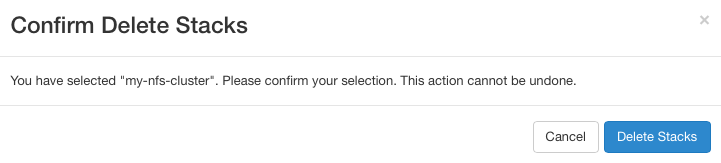
\includegraphics[width=\columnwidth]{images/chameleon/Delete-Stacks.png}

The template for the
\href{https://www.chameleoncloud.org/appliances/26/}{Hello World complex
appliance}~is~reproduced below. It is similar to the NFS share
appliance, except that it deploys only a single client. You can see that
it has four resources defined:

\begin{itemize}
\item
  nfs\_server\_floating\_ip
\item
  nfs\_server
\item
  nfs\_server\_ip\_association
\item
  nfs\_client
\end{itemize}

The nfs\_client instance mounts the NFS directory shared by the
nfs\_server instance, just like in our earlier example.

\begin{footnotesize}
\begin{verbatim}
# This describes what is deployed by this template.
description: NFS server and client deployed with Heat on Chameleon

# This defines the minimum Heat version required by this template.
heat_template_version: 2015-10-15

# The resources section defines what OpenStack resources are to be deployed and
# how they should be configured.
resources:
  nfs_server_floating_ip:
    type: OS::Nova::FloatingIP
    properties:
      pool: ext-net

  nfs_server:
    type: OS::Nova::Server
    properties:
      flavor: baremetal
      image: CC-CentOS7
      key_name: { get_param: key_name }
      networks:
         - network: sharednet1
      scheduler_hints: { reservation: { get_param: reservation_id } }
      user_data: |
        #!/bin/bash
        yum install -y nfs-utils
        mkdir -p /exports/example
        chown -R cc:cc /exports
        echo '/exports/example 10.140.80.0/22(rw,async) 10.40.0.0/23(rw,async)' >> /etc/exports
        systemctl enable rpcbind && systemctl start rpcbind
        systemctl enable nfs-server && systemctl start nfs-server

  nfs_server_ip_association:
    type: OS::Nova::FloatingIPAssociation
    properties:
      floating_ip: { get_resource: nfs_server_floating_ip }
      server_id: { get_resource: nfs_server }

  nfs_client:
    type: OS::Nova::Server
    properties:
      flavor: baremetal
      image: CC-CentOS7
      key_name: { get_param: key_name }
      networks:
         - network: sharednet1
      scheduler_hints: { reservation: { get_param: reservation_id } }
      user_data:
        str_replace:
          template: |
            #!/bin/bash
            yum install -y nfs-utils
            echo "$nfs_server_ip:/exports/example    /mnt/    nfs" > /etc/fstab
            mount -a
          params:
            $nfs_server_ip: { get_attr: [nfs_server, first_address] }

# The parameters section gathers configuration from the user.
parameters:
  key_name:
    type: string
    description: Name of a KeyPair to enable SSH access to the instance
    default: default
    constraints:
    - custom_constraint: nova.keypair
  reservation_id:
    type: string
    description: ID of the Blazar reservation to use for launching instances.
    constraints:
    - custom_constraint: blazar.reservation
\end{verbatim}
\end{footnotesize}

Download this template from the
\href{https://www.chameleoncloud.org/appliances/26/}{Hello World complex
appliance details page} to your local machine, and open it in your
favorite text editor.

We will customize~the template to add a second NFS~client by creating a
new resource called another\_nfs\_client. Add the following text to your
template inside the resources section.~Make sure to respect the level of
indentation, which is important in YAML.

\begin{footnotesize}
\begin{verbatim}
  another_nfs_client:
    type: OS::Nova::Server
    properties:
      flavor: baremetal
      image: CC-CentOS7
      key_name: { get_param: key_name }
      networks:
         - network: sharednet1
      scheduler_hints: { reservation: { get_param: reservation_id } }
      user_data:
        str_replace:
          template: |
            #!/bin/bash
            yum install -y nfs-utils
            echo "$nfs_server_ip:/exports/example    /mnt/    nfs" > /etc/fstab
            mount -a
          params:
            $nfs_server_ip: { get_attr: [nfs_server, first_address] }
\end{verbatim}
\end{footnotesize}

Now, launch a new~stack~with this~template. Since the customized
template is only on your computer and cannot be addressed by a URL, use
the ``Direct Input'' method instead and copy/paste the content of the
customized template.~The resulting topology view is shown below:~as you
can see, the two client instances are shown separately since each one is
defined as a separate resource in the template.

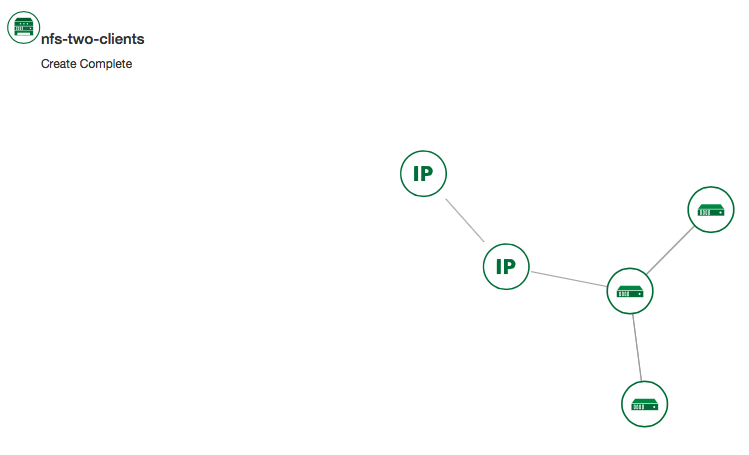
\includegraphics[width=\columnwidth]{images/chameleon/NFS-Two-Clients_lFGgizN.png}

You may have realized~already that while adding just one additional
client instance~was easy, launching more of them would require to copy /
paste blocks of YAML many times while ensuring that the total count is
correct. This would be easy to get wrong, especially when dealing with
tens or hundreds of instances.

So instead, we leverage another construct from Heat: resource groups.
Resource groups allow to define one kind of resource and request it to
be created any~number of times.

Remove the nfs\_client and another\_client resources from your
customized template, and replace them with the following:

\begin{footnotesize}
\begin{verbatim}
  nfs_clients:
    type: OS::Heat::ResourceGroup
    properties:
      count: 2
      resource_def:
        type: OS::Nova::Server
        properties:
          flavor: baremetal
          image: CC-CentOS7
          key_name: { get_param: key_name }
          networks:
             - network: sharednet1
          scheduler_hints: { reservation: { get_param: reservation_id } }
          user_data:
            str_replace:
              template: |
                #!/bin/bash
                yum install -y nfs-utils
                echo "$nfs_server_ip:/exports/example    /mnt/    nfs" > /etc/fstab
                mount -a
              params:
                $nfs_server_ip: { get_attr: [nfs_server, first_address] }
\end{verbatim}
\end{footnotesize}

A resource group is configured with a properties field, containing the
definition of the resource to launch (\texttt{resource\_def}) and the
number of resources to launch (\texttt{count}). Once launched, you will
notice that the topology view groups all client instances under a single
Resource Group icon. We use the same \texttt{resource\_def} than when
defining separate instances earlier.

Another way we can customize this template is by adding outputs to the
template. Outputs allow a Heat template to return data to the user. This
can be useful to return values like IP addresses or credentials that the
user must know to use the system.

We will create an output returning the floating IP address used by the
NFS server. We define an outputs section, and one output with the name
\texttt{server\_ip} and a description. The value of the output is
gathered using the \texttt{get\_attr} function which obtains the IP
address of the server instance.

\begin{footnotesize}
\begin{verbatim}
outputs:
  server_ip:
    description: Public IP address of the NFS server
    value: { get_attr: [nfs_server_floating_ip, ip] }
\end{verbatim}
\end{footnotesize}

You can get outputs in the ``Overview'' tab of the Stack~Details page.
If you want to use~the command line, install \texttt{python-heatclient}
and use~the \texttt{heat\ output-list} and \texttt{heat\ output-show}
commands, or get a full list in the information returned by
\texttt{heat\ stack-show}.

Multiple outputs can be defined in the outputs section. Each of them
needs to have a unique name. For example, we can add another output to
list the private IPs assigned to client instances:

\begin{footnotesize}
\begin{verbatim}
  client_ips:
    description: Private IP addresses of the NFS clients
    value: { get_attr: [nfs_clients, first_address] }
\end{verbatim}
\end{footnotesize}

The image below shows the resulting outputs as viewed from the web
interface. Of course IP addresses will be specific to each deployment.

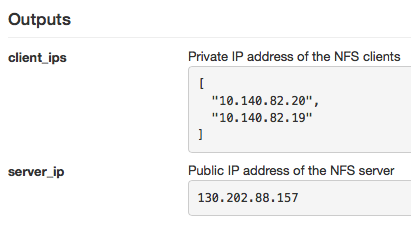
\includegraphics[width=0.5\columnwidth]{images/chameleon/Outputs.png}

Finally, we can add a new parameter to replace the hardcoded number of
client instances by a value passed to the template. Add the following
text to the parameters section:

\begin{footnotesize}
\begin{verbatim}
  nfs_client_count:
    type: number
    description: Number of NFS client instances
    default: 1
    constraints:
      - range: { min: 1 }
        description: There must be at least one client.
\end{verbatim}
\end{footnotesize}

Inside the resource group definition,
change~\texttt{count:\ 2}~to~\texttt{count:\ \{\ get\_param:\ nfs\_client\_count\ \}}~to
retrieve and use the parameter we just defined. When you launch this
template, you will see that an additional parameter allows you to define
the number of client instances, like in the NFS share~appliance.

At this stage, we have fully recreated the NFS share appliance starting
from the Hello World one! The next section will explain how to write a
new template from scratch.

\section{Writing a new template}\label{writing-a-new-template}

You may want to write a whole new template, rather than customizing an
existing one. Each template should follow the same layout and be
composed of the following sections:

\begin{itemize}
\item
  Heat template version
\item
  Description
\item
  Resources
\item
  Parameters
\item
  Outputs
\end{itemize}

\subsection{Heat template version}\label{heat-template-version}

Each Heat template has to include the heat\_template\_version key with a
valid version of HOT (Heat Orchestration Template). Chameleon bare-metal
supports any HOT version up to 2015-10-15, which corresponds to
OpenStack Liberty. The
\href{http://docs.openstack.org/developer/heat/template_guide/hot_spec.html\#hot-spec-template-version}{Heat
documentation}~lists~all available~versions and their features.~We
recommended that you always use the latest supported~version to have
access to all supported features:

\texttt{heat\_template\_version:\ 2015-10-15}

\subsection{Description}\label{description}

While not mandatory, it is good practice to describe what ~is deployed
and configured by your template. It can be on a single line:

\begin{footnotesize}
\begin{verbatim}
description: This describes what this Heat template deploys on Chameleon.
\end{verbatim}
\end{footnotesize}

If a longer description is needed, you can provide multi-line text in
YAML, for example:

\begin{footnotesize}
\begin{verbatim}
description: >
  This describes what this Heat
  template deploys on Chameleon.
\end{verbatim}
\end{footnotesize}

\subsection{Resources}\label{resources}

The resources section is required and must contain at least one resource
definition. A
\href{http://docs.openstack.org/developer/heat/template_guide/openstack.html}{complete
list of resources types known to Heat} is available.

However, only a subset of them are supported by Chameleon, and some are
limited to administrative use. We recommend that you only use:

\begin{itemize}
\item
  OS::Glance::Image
\item
  OS::Heat::ResourceGroup
\item
  OS::Heat::SoftwareConfig
\item
  OS::Heat::SoftwareDeployment
\item
  OS::Heat::SoftwareDeploymentGroup
\item
  OS::Neutron::FloatingIP
\item
  OS::Neutron::FloatingIPAssociation
\item
  OS::Neutron::Port (advanced users only)
\item
  OS::Nova::Keypair
\item
  OS::Nova::Server
\end{itemize}

If you know of another resource that you would like to use and think it
should be supported by the OpenStack services on Chameleon bare-metal,
please let us know via our help desk.

\subsection{Parameters}\label{parameters}

Parameters allow users to customize the template with necessary or
optional values. For example, they can customize which Chameleon
appliance they want to deploy, or which key pair to install. Default
values can be provided with the \texttt{default} key, as well as
constraints to ensure that only valid OpenStack resources can be
selected. For example, \texttt{custom\_constraint:\ glance.image}
restricts the image selection to an available OpenStack image, while
providing a pre-filled selection box in the web interface.
\href{http://docs.openstack.org/developer/heat/template_guide/hot_spec.html\#parameter-constraints}{More
details about constraints}~are available in the Heat documentation.

\subsection{Outputs}\label{outputs}

Outputs allow template to give information from the deployment to users.
This can include usernames, passwords, IP addresses, hostnames, paths,
etc. The outputs declaration is using the following format:

\begin{footnotesize}
\begin{verbatim}
outputs:
  first_output_name:
    description: Description of the first output
    value: first_output_value
  second_output_name:
    description: Description of the second output
    value: second_output_value
\end{verbatim}
\end{footnotesize}

Generally values will be calls to get\_attr, get\_param, or some other
function to get information from parameters or resources deployed by the
template and return them in the proper format to the user.

\section{Sharing new complex
appliances}\label{sharing-new-complex-appliances}

If you have written your own complex appliances
or~substantially~customized an existing one, we would love if you shared
them with our user community!

The process is very similar to regular appliances: log into the
Chameleon portal, go to the
\href{https://www.chameleoncloud.org/appliances/}{appliance catalog},
and click on the button in the top-right corner: ``Add an appliance''
(you need to be logged in to see it).


\includegraphics[width=0.25\columnwidth]{images/chameleon/Add-an-appliance.png}

You will be prompted to enter a name, description, and documentation.
Instead of providing appliance IDs, copy your template to the dedicated
field. Finally, share your contact information and assign a version
string to your appliance. Once submitted, your appliance will be
reviewed. We will get in touch if a change is needed, but if it's all
good we will publish it right away!

\section{Advanced topics}\label{advanced-topics}

\subsection{All-to-all information
exchange}\label{all-to-all-information-exchange}

The previous examples have all used user-data scripts to provide
instances with contextualization information. While it is easy to use,
this contextualization method has a major drawback: because it is given
to the instance as part of its launch request, it cannot use any context
information that is not yet known at this time.

In practice, this means that in a client-server deployment, only one of
these pattern will be possible:

\begin{itemize}
\item
  The server has to be deployed first, and once it is deployed, the
  clients can be launched and contextualized with information from the
  server. The server won't know about the clients unless there is a
  mechanism (not managed by Heat) for the client to contact the server.
\item
  The clients have to be deployed first, and once they are deployed, the
  server can be launched and contextualized with information from the
  clients. The clients won't know about the server unless there is a
  mechanism (not managed by Heat) for the server to contact the clients.
\end{itemize}

This limitation was already apparent in our NFS share~appliance: this is
why the server instance exports the file system to all bare-metal
instances on Chameleon, because it doesn't know which specific IP
addresses are allocated to the clients.

This limitation is even more important if the deployment is not
hierarchical, i.e. all instances need to know about all others. For
example, a cluster with IP and hostnames populated in /etc/hosts
required each instance to be known by every other instance.

This section presents a more advanced form of contextualization that can
perform this kind of information exchange. This is implemented by Heat
agents running inside instances and communicating with the Heat service
to send and receive information. This means you will need to use an
image bundling these agents. Currently, our CC-CentOS7 appliance and its
CUDA version are the only ones supporting this mode of
contextualization. If you build your own images using the
\href{https://github.com/ChameleonCloud/CC-CentOS7}{CC-CentOS7 appliance
builder}, you will automatically have these agents installed.

This contextualization is performed with several Heat resources:

\begin{itemize}
\item
  \texttt{OS::Heat::SoftwareConfig}.~This resource describes code to run
  on an instance. It can be configured with inputs and provide outputs.
\item
  \texttt{OS::Heat::SoftwareDeployment}. This resource applies a
  SoftwareConfig to a specific instance.
\item
  \texttt{OS::Heat::SoftwareDeploymentGroup}. This resource applies a
  SoftwareConfig to a specific group of instances.
\end{itemize}

The template below illustrates how it works. It launches a group of
instances that will automatically populates their /etc/hosts file with
IP and hostnames from other instances in the deployment.

\begin{footnotesize}
\begin{verbatim}
heat_template_version: 2015-10-15

description: >
  This template demonstrates how to exchange hostnames and IP addresses to populate /etc/hosts.

parameters:
  flavor:
    type: string
    default: baremetal
    constraints:
    - custom_constraint: nova.flavor
  image:
    type: string
    default: CC-CentOS7
    constraints:
    - custom_constraint: glance.image
  key_name:
    type: string
    default: default
    constraints:
    - custom_constraint: nova.keypair
  instance_count:
    type: number
    default: 2
  reservation_id:
    type: string
    description: ID of the Blazar reservation to use for launching instances.
    constraints:
    - custom_constraint: blazar.reservation

resources:
  export_hosts:
    type: OS::Heat::SoftwareConfig
    properties:
      outputs:
        - name: hosts
      group: script
      config: |
        #!/bin/sh
        (echo -n $(facter ipaddress); echo -n ' '; echo $(facter hostname)) > ${heat_outputs_path}.hosts

  export_hosts_sdg:
    type: OS::Heat::SoftwareDeploymentGroup
    properties:
      config: { get_resource: export_hosts }
      servers: { get_attr: [server_group, refs_map] }
      signal_transport: HEAT_SIGNAL

  populate_hosts:
    type: OS::Heat::SoftwareConfig
    properties:
      inputs:
        - name: hosts
      group: script
      config: |
        #!/usr/bin/env python
        import ast
        import os
        import string
        import subprocess
        hosts = os.getenv('hosts')
        if hosts is not None:
            hosts = ast.literal_eval(string.replace(hosts, '\n', '\\n'))
        with open('/etc/hosts', 'a') as hosts_file:
          for ip_host in hosts.values():
              hosts_file.write(ip_host.rstrip() + '\n')

  populate_hosts_sdg:
    type: OS::Heat::SoftwareDeploymentGroup
    depends_on: export_hosts_sdg
    properties:
      config: { get_resource: populate_hosts }
      servers: { get_attr: [server_group, refs_map] }
      signal_transport: HEAT_SIGNAL
      input_values:
        hosts: { get_attr: [ export_hosts_sdg, hosts ] }

  server_group:
    type: OS::Heat::ResourceGroup
    properties:
      count: { get_param: instance_count }
      resource_def:
        type: OS::Nova::Server
        properties:
          flavor: { get_param: flavor }
          image: { get_param: image }
          key_name: { get_param: key_name }
          networks:
             - network: sharednet1
          scheduler_hints: { reservation: { get_param: reservation_id } }
          user_data_format: SOFTWARE_CONFIG
          software_config_transport: POLL_SERVER_HEAT

outputs:
  deployment_results:
    value: { get_attr: [export_hosts_sdg, hosts] }
\end{verbatim}
\end{footnotesize}

There are two SoftwareConfig resources.

The first SoftwareConfig, export\_hosts, uses the facter tool to extract
IP address and hostname into a single line (in the format expected for
/etc/hosts) and writes it to a special path
(\$\{heat\_outputs\_path\}.hosts). This prompts Heat to assign the
content of this file to the output with the name hosts.

The second SoftwareConfig, populate\_hosts, takes as input a variable
named hosts, and applies a script that reads the variable from the
environment, parses it with ast.literal\_eval (as it is formatted as a
Python dict), and writes each value of the dictionary to /etc/hosts.

The SoftwareDeploymentGroup resources export\_hosts\_sdg and
populate\_hosts\_sdg apply each SoftwareConfig to the instance
ResourceGroup with the correct configuration.

Finally, the instance ResourceGroup is configured so that each instance
uses the following contextualization method instead of a user-data
script:

\begin{footnotesize}
\begin{verbatim}
          user_data_format: SOFTWARE_CONFIG
          software_config_transport: POLL_SERVER_HEAT
\end{verbatim}
\end{footnotesize}

You can follow the same template pattern to configure your own
deployment requiring all-to-all information exchange.



\FILENAME

\section{Bare Metal}\label{C:cc-baremetal}

In this page you will find documentation guiding you through the
bare-metal deployment features available in~Chameleon. Chameleon gives
users administrative access to bare-metal compute resources to
run~{cloud computing~}experiments with a high degree of customization
and repeatability. Typically, an experiment will go through several
phases, as illustrated in the figure below:


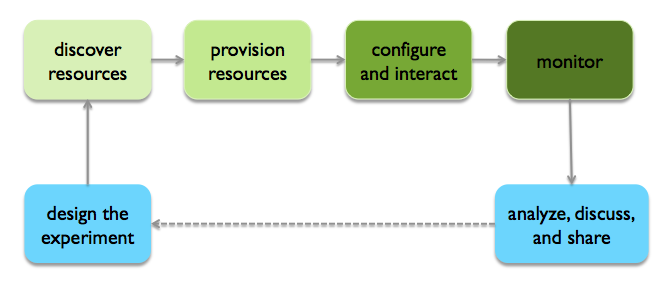
\includegraphics[width=\columnwidth]{images/chameleon/baremetal.png}


The bare-metal user guide comes in two editions. The first is how to use
Chameleon resources~via the web interface, the recommended choice for
new users to quickly learn how to use our testbed:

\textbf{\href{https://www.chameleoncloud.org/discover-resources}{Get
started with Chamelon using the web interface}}

\begin{enumerate}
\item
  \href{https://www.chameleoncloud.org/discover-resources/}{Discover
  Resources}
\item
  \href{https://www.chameleoncloud.org/provision-resources/}{Provision
  Resources}~
\item
  \href{https://www.chameleoncloud.org/configure-and-interact/}{Configure
  and Interact}
\item
  \href{https://www.chameleoncloud.org/monitor-and-collect/}{Monitor and
  Collect Results}
\end{enumerate}

The second targets~advanced users who are already familiar with
Chameleon~and would like to learn how to use Chameleon from the~command
line or with scripts.

\href{https://www.chameleoncloud.org/discover-resources-command-lines}{Get
started with Chameleon using the command line~(advanced)}

\begin{enumerate}
\item
  \href{https://www.chameleoncloud.org/discover-resources-command-lines/}{Discover
  Resources}
\item
  \href{https://www.chameleoncloud.org/advanced-provision-resources/}{Provision
  Resources}
\item
  \href{https://www.chameleoncloud.org/advanced-configure-and-interact/}{Configure
  and Interact}
\item
  \href{https://www.chameleoncloud.org/monitor-and-collect/}{Monitor and
  Collect Results}
\end{enumerate}

You do not need to strictly follow the documentation~sequentially.
However, note that some steps assume that~previous ones have been
successfully performed.

You can also consult~documentation~describing how to use advanced
features of Chameleon not covered by the guides above:

\begin{itemize}
\item
  the
  \href{https://www.chameleoncloud.org/docs/bare-metal-user-guide/chameleon-object-store/}{Chameleon
  Object Store},
\item
  \href{https://www.chameleoncloud.org/docs/bare-metal-user-guide/network-isolation-bare-metal/}{network
  isolation for bare metal}.
\end{itemize}





\section{Frequently Asked Questions}\label{frequently-asked-questions}

\FILENAME

\subsection{Appliances}\label{appliances}

\subsubsection{What is an appliance?}\label{what-is-an-appliance}

An appliance is an application packaged together with the environment
that this application requires. For example, an appliance can consists
of the operating system, libraries and tools used by the application,
configuration features such as environment variable settings, and the
installation of the application itself. Examples of appliances might
include a KVM virtual machine image, a Docker image, or a bare metal
image. Chameleon appliance refers to bare metal images that can be
deployed on the Chameleon testbed. Since an appliance captures the
experimental environment exactly, it is a key element of
reproducibility; publishing an appliance used to obtain experimental
results will go a long way to allowing others to reproduce and build on
your research easily.

To deploy distributed applications on several Chameleon instances,
complex appliances combine an image and a template describing how the
cluster should be configured and contextualized. You can read more about
them in the
\href{https://www.chameleoncloud.org/docs/complex-appliances/}{Complex
Appliances documentation}.

\subsubsection{What is the Appliance Catalog?}\label{what-is-the-chameleon-appliance-catalog}

\href{https://www.chameleoncloud.org/appliances/}{The Chameleon
Appliance Catalog} is a repository that allows users to discover,
publish, and share appliances. The appliance catalog contains useful
images of both bare metal and virtual machine appliances supported by
the Chameleon team as well appliances contributed by users.

\subsubsection{How do I publish an appliance in the Appliance Catalog?}\label{how-do-i-publish-an-appliance-in-the-chameleon-appliance-catalog}

The new Appliance Catalog allows you to easily publish and share your
own appliances so that others can discover them and use them either to
reproduce the research of others or as a basis for their own research.
 Before creating your own appliance it is advisable to review other
appliances on
the \href{https://www.chameleoncloud.org/appliances/}{Chameleon
Appliance Catalog} in order to get an idea of the categories you will
want to contribute and what others have done. 

Once you are ready to proceed, an appliance can be contributed to
Chameleon in the following steps:

\begin{enumerate}

\item
  Create the appliance itself. You may want to test it as well as give
  some thought to what support you are willing to provide for the
  appliance (e.g., if your group developed and supports a software
  package, the appliance may be just a new way of packaging the software
  and making it available, in which case your standard support channels
  may be appropriate for the appliance as well).
\item
  Upload the appliance to the Chameleon Image Repository (Glance) and
  make the image public. In order to enter the appliance into the
  Catalog you will be asked to provide the Glance ID for the image.
  These IDs are per-cloud, so that there are three options right now:
  bare metal/CHI at University of Chicago, bare metal/CHI at TACC, and
  OpenStack/KVM at TACC. You will need to provide at least one
  appliance, but may want to provide all three.
\item
  Go to
  the \href{https://www.chameleoncloud.org/appliances/create/}{Appliance
  Catalog Create Appliance web form}, fill out, and submit the form. Be
  prepared to provide the following information: a descriptive name
  (this sometimes requires some thought!), author and support contact,
  version, and an informative description. The description is a very
  important part of the appliance record; others will use it to evaluate
  if the appliance contains tools they need for their research so it
  makes sense to prepare it carefully. To make your description
  effective you may want to think of the following questions: what does
  the appliance contain? what are the specific packages and their
  versions? what is it useful for? where can it be deployed and/or what
  restrictions/limitations does it have? how should users connect to it
  / what accounts are enabled?
\end{enumerate}

If you are adding a complex appliance, skip the image ID fields and
enter your template instead in the dedicated text box.

As always, if you encounter any problems or want to share with us
additional improvements we should do to the process, please don't
hesitate to \href{https://www.chameleoncloud.org/help/}{submit a
ticket}. 

\subsubsection{How can I manage an appliance on Appliance
Catalog?}\label{how-can-i-manage-an-appliance-on-chameleon-appliance-catalog}

If you are the owner of the appliance, you can edit the appliance
data, such as the description or the support information. Browse to the
appliance that you want to edit and view its Details page. At the top
right of the page is an Edit button. You will be presented with the same
web form as when creating the appliance, pre-filled with the appliances
current information. Make changes as necessary and click Save at the
bottom of the page.

And finally, you can delete appliances you had made available. {Browse
to the appliance that you want to delete and click Edit on the
Appliance Details page. At the bottom of the page is a Delete button.
You will be asked to confirm once more that you do want to delete this
appliance}. After confirming, the appliance will be removed and no
longer listed on the Appliance Catalog.

\subsubsection{Why are there different image IDs  for the same
appliance?}\label{why-are-there-different-image-ids-for-kvmtacc-chitacc-and-chiuc-for-the-same-appliance}

The three clouds forming the Chameleon testbed are fully separated, each
having its own Glance image repository. The same appliance
image uploaded to the three clouds will produce three different image
IDs.

In addition, it is sometimes needed to customize an appliance image for
each site, resulting in slightly different image files.

\subsubsection{Can I use another operating system on bare-metal?}\label{can-i-useubuntudebian-oranother-operating-system-rather-than-centos-on-bare-metal}

The recommended appliance for Chameleon is CentOS 7 (supported by
Chameleon staff), or appliances built on top of it.\\
These appliances provide Chameleon-specific customizations, such as
login using the cc account, the cc-checks utility to verify hardware
against our resource registry, gathering of metrics, etc.

Since 2016, we also provide and support Ubuntu 14.04 and
16.04 appliances with the same functionality.

\subsection{Bare Metal Troubleshooting}\label{bare-metal-troubleshooting}

\subsubsection{Why are my Bare Metal instances failing to
launch?}\label{why-are-my-bare-metal-instances-failing-to-launch}

The Chameleon Bare Metal clouds require users to reserve resources
before allowing them to launch instances. Please follow the
\href{https://www.chameleoncloud.org/docs/bare-metal/}{documentation}
and make sure that:

\begin{enumerate}
\item
  You have created a lease and it has started (the associated
  reservation is shown as \textbf{Active})
\item
  You have selected your reservation in the \textbf{Launch Instance}
  panel
\end{enumerate}

If you still cannot start instances, please
\href{https://www.chameleoncloud.org/user/help/}{open a ticket with our
help desk}.

\subsection{OpenStack KVM Troubleshooting}\label{openstack-kvm-troubleshooting}

\subsubsection{Why are my OpenStack KVM instances failing to
launch?}\label{why-are-my-openstack-kvm-instances-failing-to-launch}

If you get an error stating that \textbf{No valid host was found}, it
might be caused by a lack of resources in the cloud. The Chameleon staff
continuously monitors the utilization of the testbed, but there might be
times when no more resources are available. If the error persists,
please \href{https://www.chameleoncloud.org/user/help/}{open a ticket
with our help desk}.

\subsubsection{Why can't I ping or SSH to my
instance?}\label{why-cant-i-ping-or-ssh-to-my-instance}

While the possibility that the system is being taking over by nanites
should not be discounted too easily, it is always prudent to first
check for the following issues:

\begin{itemize}
\item
  Do you have a floating IP associated with your instance? By default,
  instances do not have publicly-accessible IP addresses assigned. See
  the \textbf{Managing Virtual Machine Instances} section in the
  \href{https://www.chameleoncloud.org/docs/user-guides/openstack-kvm-user-guide/}{User
  Guide}.
\item
  Does your security group allow incoming ICMP (e.g. ping) traffic? By
  default, firewall rules do not allow ping to your instances. If you
  wish to enable it, see the \textbf{Firewall (Access Security)} section
  in the
  \href{https://www.chameleoncloud.org/docs/user-guides/openstack-kvm-user-guide/}{User
  Guide}.
\item
  Does your security group allow incoming SSH (TCP port 22) traffic? By
  default, firewall rules do not allow SSH to your instances. If you
  wish to enable it, see the \textbf{Firewall (Access Security)} section
  in the
  \href{https://www.chameleoncloud.org/docs/user-guides/openstack-kvm-user-guide/}{User
  Guide}.
\end{itemize}

 If none of these solve your problem,
please \href{https://www.chameleoncloud.org/user/help/}{open a ticket
with our help desk}, and send us the results of the above (and any
evidence of nanites you find as well).



